\documentclass[sigplan,screen]{acmart}
%\settopmatter{authorsperrow=4}

%replace XXX with the submission number you are given from the ASPLOS submission site.
\newcommand{\asplossubmissionnumber}{324}

\hypersetup{
	colorlinks=true,
}

% AA: I need this so that the 'fi' ligature in the pdfs compiles correctly on my machine.
\pdfmapline{-dummy LMRoman10-Regular}

% Uncomment to show margins
% \usepackage{showframe}

\usepackage{balance}
\setlength{\paperheight}{11in}
\usepackage{graphicx}
\usepackage{multirow}
\usepackage{ifthen}
\usepackage{color}
\usepackage[normalem]{ulem}
\usepackage{hhline}
\usepackage{xcolor,colortbl}
\usepackage{alltt}
\usepackage{amssymb}
\usepackage{enumitem}
\usepackage{breakcites}
\usepackage{microtype}
\usepackage{flushend} 	% It balance references in the last page, but it has a bug
% to display a last reference.
\usepackage{xspace}
\usepackage{booktabs}
\usepackage{rotating}
\usepackage{float}
\usepackage{siunitx}
\usepackage{dcolumn}
% \usepackage{textcomp}

\usepackage{array}
\usepackage{booktabs}
\usepackage{tabularx}
\usepackage{tabulary}
\usepackage{makecell}

\usepackage{wrapfig}
\usepackage{comment}
% \usepackage[hyphens]{url} % break lines at hyphens
\usepackage{adjustbox}
\usepackage{ragged2e}
\usepackage{pifont}
\usepackage{amsmath}
\usepackage{changepage}
%\usepackage[kerning=true,spacing=true]{microtype}
%\usepackage{microtype}
\usepackage[font=small,labelfont=bf]{caption}
\usepackage{placeins}
%\usepackage[sort]{natbib} % sort option relplaces cite package
%\usepackage[sort&compress]{natbib}
% Don't use titling with acmart.cls
% \usepackage{titling}
\usepackage{setspace}

% \usepackage[
% colorlinks,linkcolor={black},citecolor={black},
% urlcolor={black}
% ]
% {hyperref}

\usepackage{float}
\usepackage{tikz}
\usepackage{pgfplots}
\def\checkmark{\tikz\fill[scale=0.4](0,.35) -- (.25,0) -- (1,.7) -- (.25,.15) -- cycle;}
\newcommand{\cross}{$\mathbin{\tikz [x=1.4ex,y=1.4ex,line width=.2ex] \draw (0,0) -- (1,1) (0,1) -- (1,0);}$}%

\usepackage[T1]{fontenc}

\renewcommand{\ttdefault}{txtt}
% YAML highlight
%\usepackage[dvipsnames]{xcolor}
\usepackage{listings}
\lstset{
	literate={\_}{}{0\discretionary{\_}{}{\_}}%
}

\newcommand*{\origrightarrow}{}
\let\oldarrow\textrightarrow
\renewcommand*{\textrightarrow}{\fontfamily{cmr}\selectfont\origrightarrow}
%\setlength{\belowcaptionskip}{-10pt} % -10pt is the best

%%%%%%%%%%%%%%%%%%%%%%%%%%
%%% SPACE SQUEEZE STUFF
%%% TRY NOT TO USE!
%%%%%%%%%%%%%%%%%%%%%%%%%%
\newboolean{squeeze}
\setboolean{squeeze}{true}
%\setboolean{squeeze}{false}
\ifthenelse{\boolean{squeeze}}{
  %\renewcommand{\baselinestretch}{0.99} % VM: Taking this out for now to improve readability
  \setlength{\textfloatsep}{1ex plus 1ex minus .2ex}
  \setlength{\intextsep}{1ex plus 1ex minus .2ex}
  \setlength{\floatsep}{1ex plus 1ex minus .2ex}
  \captionsetup[table]{belowskip=0pt,aboveskip=0pt}
  \captionsetup[figure]{belowskip=0pt,aboveskip=5pt}

  \widowpenalty=25
  \clubpenalty=25
}{}


%%%%%%%%%%%%%%%%%%%%%%%%%%
%%% SQUEEZE \section
%%%%%%%%%%%%%%%%%%%%%%%%%%
\makeatletter
\let\orig@section\section
\newcommand{\@sectionstar}[1]{\vspace{-0.5\baselineskip}\orig@section*{#1}\vspace{-0.2pt}}
\newcommand{\@sectionnostar}[1]{\vspace{-0.5\baselineskip}\orig@section{#1}\vspace{-0.2pt}}
\renewcommand{\section}{\@ifstar{\@sectionstar}{\@sectionnostar}}
\makeatother

%%%%%%%%%%%%%%%%%%%%%%%%%%
%%% SQUEEZE \subsection
%%%%%%%%%%%%%%%%%%%%%%%%%%
\makeatletter
\let\orig@subsection\subsection
\renewcommand{\subsection}[1]{\vspace{-0.5\baselineskip}\orig@subsection{#1}\vspace{-0.35pt}}
\makeatother

%%%%%%%%%%%%%%%%%%%%%%%%%%
%%% SQUEEZE bib
%%%%%%%%%%%%%%%%%%%%%%%%%%
\let\oldbibliography\thebibliography
\renewcommand{\thebibliography}[1]{\oldbibliography{#1}
	\setlength{\itemsep}{0pt}}

\newcommand\T{\rule{0pt}{2.0ex}}
\newcommand\B{\rule[-0.9ex]{0pt}{0pt}}
\newcommand{\fs}[1]{\footnotesize{#1}}
\newcommand{\bfs}[1]{\textbf{\footnotesize{#1}}}
% \newcommand{\mrot}[1]{\begin{rotate}{55}{\bfs{#1}}\end{rotate}}
% \newcommand{\rot}[1]{\begin{rotate}{90}{\bfs{#1}}\end{rotate}}

%% ---------------------------------------
%% change this to hide/show the grumblers
%% and ``for our eyes only'' sections
%% ---------------------------------------

\newboolean{publicversion}
%\setboolean{publicversion}{false}
\setboolean{publicversion}{true}

\newboolean{changecoloring}
%\setboolean{changecoloring}{false}
\setboolean{changecoloring}{true}

\newboolean{tinypolishing}
\setboolean{tinypolishing}{false}

\colorlet{changecoloringtmp}{black}
\ifthenelse{\boolean{changecoloring}}{
  \DeclareCaptionFont{unchangedcaptionfont}{\color{gray}}
  \DeclareCaptionFont{changedcaptionfont}{\color{black}}

  \newcommand*{\beginunchanged}{%
  \colorlet{changecoloringtmp}{.}%
  \color{gray}%
  \captionsetup{labelfont={unchangedcaptionfont,bf},textfont=unchangedcaptionfont}%
  \let\changecoloringtmpgrumbler\grumbler
  \def\grumbler{}}

  \newcommand*{\beginchanged}{%
  \color{changecoloringtmp}%
  \captionsetup{labelfont={changedcaptionfont,bf},textfont=changedcaptionfont}%
  \let\grumbler\changecoloringtmpgrumbler}
}{
  \newcommand*{\beginunchanged}{}
  \newcommand*{\beginchanged}{}
}

\ifthenelse{\boolean{publicversion}}{
  \newcommand{\polishing}[1]{}
}{
\ifthenelse{\boolean{tinypolishing}}{
  \newcommand{\polishing}[1]{\bgroup#1\egroup}
}{
  \newcommand{\polishing}[1]{\bgroup\def\bf{} Polishing: #1\egroup}
}
}

\ifthenelse{\boolean{publicversion}}{
	\newcommand{\grumbler}[3]{}
}{
	\newcommand{\grumbler}[3]{\textcolor{#3}{\bf #1: #2}}
}

% Add your own...
\newcommand{\cjr}[1]{\grumbler{CJR}{#1}{blue}}
\newcommand{\hyu}[1]{\grumbler{HYU}{#1}{YellowOrange}}
\newcommand{\aak}[1]{\grumbler{AA}{#1}{violet}}
\newcommand{\amp}[1]{\grumbler{AMP}{#1}{purple}}
\newcommand{\review}[1]{\grumbler{Reviewer}{#1}{red}}
\newcommand{\reviewer}[2]{\grumbler{Reviewer\##1}{#2}{red}}

\newcommand{\newterm}[1]{{\bf #1}}
\newcommand{\parname}[1]{\textbf{\textit{#1}}}
\newcommand{\paragraphbe}[1]{\vspace{.25ex}\noindent\parname{#1} }

% This macro that I got off stackexchange is supposed to help LaTeX understand how to break
% URLs nicely across lines.
% https://tex.stackexchange.com/a/10401
\expandafter\def\expandafter\UrlBreaks\expandafter{\UrlBreaks
  \do\a\do\b\do\c\do\d\do\e\do\f\do\g\do\h\do\i\do\j
  \do\k\do\l\do\m\do\n\do\o\do\p\do\q\do\r\do\s\do\t
  \do\u\do\v\do\w\do\x\do\y\do\z\do\A\do\B\do\C\do\D
  \do\E\do\F\do\G\do\H\do\I\do\J\do\K\do\L\do\M\do\N
  \do\O\do\P\do\Q\do\R\do\S\do\T\do\U\do\V\do\W\do\X
  \do\Y\do\Z}

\input{terminology}

% YAML highlight
\newcommand\YAMLcolonstyle{\color{red}\mdseries}
\newcommand\YAMLkeystyle{\color{black}\bfseries}
\newcommand\YAMLvaluestyle{\color{blue}\mdseries}

\makeatletter
% here is a macro expanding to the name of the language
% (handy if you decide to change it further down the road)
\newcommand\language@yaml{yaml}
\expandafter\expandafter\expandafter\lstdefinelanguage
\expandafter{\language@yaml}
{
	keywords={true,false,null,y,n},
	keywordstyle=\color{darkgray}\bfseries,
	basicstyle=\YAMLkeystyle,                                 % assuming a key comes first
	sensitive=false,
	comment=[l]{\#},
	morecomment=[s]{/*}{*/},
	commentstyle=\color{purple}\ttfamily,
	stringstyle=\YAMLvaluestyle\ttfamily,
	moredelim=[l][\color{orange}]{\&},
	moredelim=[l][\color{magenta}]{*},
	moredelim=**[il][\YAMLcolonstyle{:}\YAMLvaluestyle]{:},   % switch to value style at :
	morestring=[b]',
	morestring=[b]",
	literate =    {---}{{\ProcessThreeDashes}}3
	{>}{{\textcolor{red}\textgreater}}1
	{|}{{\textcolor{red}\textbar}}1
	{\ -\ }{{\mdseries\ -\ }}3,
}

% switch to key style at EOL
\lst@AddToHook{EveryLine}{\ifx\lst@language\language@yaml\YAMLkeystyle\fi}

\newcommand{\elidedcodeStart}[1]{\bgroup\itshape\color{black!60!green}[\aftergroup\elidedcodeEnd}
\def\elidedcodeEnd{]\egroup}
\newcommand{\elidedcode}[1]{\text{\itshape\color{black!60!green}...{#1}...}}
    
\makeatother

\lstset{
	breaklines=true,
	basicstyle={\small\ttfamily},
	literate={*}{{\fontfamily{lmtt}\selectfont*}}1,
	numbers=left,
	numberstyle=\scriptsize\color{gray!50!black},
	commentstyle=\itshape\color{black!60!green},
	%stepnumber=1,
	numbersep=4pt,
    moredelim={**[is][\lapisprototypestyle]{@@}{@@}},
    escapechar=|
}

% http://tex.stackexchange.com/q/43526
% fix the apparently deliberate but undocumented behaviour of disabling escapes other than mathescape in TextStyle (used by \lstinline)
% there may be a good reason why this is disabled by default, so beware in case it causes any problems
\usepackage{etoolbox}
\makeatletter
\patchcmd{\lsthk@TextStyle}{\let\lst@DefEsc\@empty}{}{}{\errmessage{failed to patch}}
\makeatother

% The box macro in case we need it

%\usepackage{tikz}
%\makeatletter
%\newcommand{\bt@HL@box}[2][]{%
%    \tikz[#1]{%
%        \pgfpathrectangle{\pgfpoint{1pt}{0pt}}{\pgfpoint{\wd #2}{\ht #2}}%
%        \pgfusepath{use as bounding box}%
%        \node[anchor=base west, outer sep=0pt,inner xsep=1pt, inner ysep=0pt, rounded corners=1pt, minimum height=\ht\strutbox+1pt,#1]{\raisebox{1pt}{\strut}\strut\usebox{#2}};
%    }%
%}
%\newenvironment{btHighlight}[1][]
%{\begingroup\tikzset{bt@Highlight@par/.style={#1}}\begin{lrbox}{\@tempboxa}}
%    {\end{lrbox}\bt@HL@box[bt@Highlight@par]{\@tempboxa}\endgroup}
%
%\newcommand\btHL[1][]{%
%    \begin{btHighlight}[#1]\bgroup\aftergroup\bt@HL@endenv%
%}
%\def\bt@HL@endenv{%
%    \end{btHighlight}%
%    \egroup
%}
%\makeatother

% Due to how lstlisting works, this works better if it SETs the style instead of styling and argument.
\newcommand*{\lapiskeywordstyle}{\color{blue!50!black}\bfseries}
\newcommand*{\lapisstdlibstyle}{\color{green!40!black}\itshape}
\newcommand*{\lapisprototypestyle}{\color{black!70}}


\lstdefinestyle{nwspecc}{
	breaklines=true,
	language=C,
    % This intentionally replaces all normal C keywords, since they are not the important part of nwspecc listings.
    keywords={},
    % API remoting related Lapis keywords
    emph={[1]sync,async,name,version,identifier,opaque,
          number,export_qualifier,success,type,in,out,buffer,
          zerocopy,type_cast,
          element,allocates,deallocates,argument,
          handle,callback,userdata,return_value,field,
          contextual_argument,
          lifetime_manual,lifetime_call,allocate,deallocate,no_copy,
          index,policy,
          utility},
          % \btHL[fill=blue!10,draw=blue!50!black]
    emphstyle={[1]\lapiskeywordstyle},
    % Resource accounting related Lapis keywords
    emph={[2]throughput_rc,consumes_rc,allocates_rc,deallocates_rc,
              continuous_rc,instantaneous_rc},
    emphstyle={[2]\lapiskeywordstyle},
    % Record-and-replay related Lapis keywords
    emph={[3]obj_record,obj_depends_on,obj_state_cbs},
    emphstyle={[3]\lapiskeywordstyle},
    % Standard library
    emph={[4]buf_registry,register_buf,get_bufs,get_n_bufs,get_buf_size,
        declare_metadata,metadata,
        strlen,min,max,
        zerocopy_alloc,zerocopy_free,zerocopy_get_physical_address},
    emphstyle={[4]\lapisstdlibstyle},
    moredelim={**[is][\lapisprototypestyle]{@@}{@@}}
}

%
% Table
\newcolumntype{P}[1]{>{\centering\arraybackslash}p{#1}}
\newcolumntype{M}[1]{>{\centering\arraybackslash}m{#1}}

\newcommand\ProcessThreeDashes{\llap{\color{cyan}\mdseries-{-}-}}
%\setlength{\bibsep}{2.5pt}

%
% defining the \BibTeX command - from Oren Patashnik's original BibTeX documentation.
\def\BibTeX{{\rm B\kern-.05em{\sc i\kern-.025em b}\kern-.08emT\kern-.1667em\lower.7ex\hbox{E}\kern-.125emX}}

%%
%% \BibTeX command to typeset BibTeX logo in the docs
\AtBeginDocument{%
	\providecommand\BibTeX{{%
			\normalfont B\kern-0.5em{\scshape i\kern-0.25em b}\kern-0.8em\TeX}}}

%% Rights management information.  This information is sent to you
%% when you complete the rights form.  These commands have SAMPLE
%% values in them; it is your responsibility as an author to replace
%% the commands and values with those provided to you when you
%% complete the rights form.
\copyrightyear{2020}
\acmYear{2020}
\setcopyright{acmcopyright}
\acmConference[ASPLOS '20]{Proceedings of the Twenty-Fifth International Conference on Architectural Support for Programming Languages and Operating Systems}{March 16--20, 2020}{Lausanne, Switzerland}
\acmBooktitle{Proceedings of the Twenty-Fifth International Conference on Architectural Support for Programming Languages and Operating Systems (ASPLOS '20), March 16--20, 2020, Lausanne, Switzerland}
\acmPrice{15.00}
\acmDOI{10.1145/3373376.3378466}
\acmISBN{978-1-4503-7102-5/20/03}

\fancyhead{}

%
% end of the preamble, start of the body of the document source.
\begin{document}

% !TeX root = proposal.tex
\begin{abstract}
The proposed dissertation will focus on developer effort and compatibility in
software virtualization of CPU ISAs, and software virtualization of
specialized compute devices (e.g., GPUs, TPUs) that are programmed through an
API.

Although binary translation is a well-established software ISA virtualization
technique, given the size and complexity of today's dominant ISAs, developers
are routinely forced to adopt ad-hoc techniques to prioritize development
effort. The proposed dissertation will present a principled approach to
determine priority among different parts of the ISA. We believe this data will
be useful to designers of virtual ISAs as well.

Specialized compute accelerators, such as GPUs and TPUs, are usually
controlled through a user-space API.
The proposed dissertation will show that unlike with CPUs, where the ISA is
the canonical interface provided to the programmer, ISA virtualization is
untenable for specialized compute accelerators. Further, the proposed
dissertation will present a present a novel taxonomy, \emph{IEMTS} for cleanly
understanding the design space for virtualizing compute accelerators.
Based on insights from this taxonomy, the proposed dissertation will
present a novel virtualization technique, \emph{hypervisor-mediated
API-remoting}, that is at once realizable and performant.
\end{abstract}

%\title{Accelerator Virtualization with \model}
%\title{Hypervisor-level Accelerator Virtualization via Language and Compiler Support}
%\title{Language and Compiler-Assisted Hypervisor-level Accelerator Virtualization}
%\title{Automatic Virtualization of Accelerators with \model}
\title{\model: Accelerated Virtualization of Accelerators}

\begin{comment}
\author{Hangchen Yu}
\affiliation{%
	\institution{The University of Texas at Austin}
}
\email{hyu@cs.utexas.edu}

\author{Arthur M. Peters}
\affiliation{%
	\institution{The University of Texas at Austin}
}
\email{amp@cs.utexas.edu}

\author{Amogh Akshintala}
\affiliation{%
	\institution{The University of North Carolina at Chapel Hill}
}
\email{aakshintala@cs.unc.edu}

\author{Christopher J. Rossbach}
\affiliation{%
	\institution{The University of Texas at Austin and VMware Research}
}
\email{rossbach@cs.utexas.edu}
\end{comment}

\author{Hangchen Yu$^{\dagger}$, Arthur Michener Peters$^{\dagger}$, Amogh Akshintala$^{\mathsection}$, Christopher J. Rossbach$^{\dagger\mathparagraph}$}
\affiliation{
	\institution{$^{\dagger}$The University of Texas at Austin, $^{\mathsection}$The University of North Carolina at Chapel Hill, $^{\mathparagraph}$VMware Research}
}
\email{{hyu,amp}@cs.utexas.edu,  aakshintala@cs.unc.edu,  rossbach@cs.utexas.edu}

\begin{CCSXML}
	<ccs2012>
	<concept>
	<concept_id>10011007.10010940.10010941.10010942.10010948</concept_id>
	<concept_desc>Software and its engineering~Virtual machines</concept_desc>
	<concept_significance>500</concept_significance>
	</concept>
	<concept>
	<concept_id>10011007.10010940.10010941.10010949</concept_id>
	<concept_desc>Software and its engineering~Operating systems</concept_desc>
	<concept_significance>300</concept_significance>
	</concept>
	<concept>
	<concept_id>10011007.10011006.10011041.10011047</concept_id>
	<concept_desc>Software and its engineering~Source code generation</concept_desc>
	<concept_significance>300</concept_significance>
	</concept>
	</ccs2012>
\end{CCSXML}

\ccsdesc[500]{Software and its engineering~Virtual machines}
\ccsdesc[300]{Software and its engineering~Operating systems}
\ccsdesc[300]{Software and its engineering~Source code generation}

\keywords{Virtualization, Code generation}

%\date{}
\renewcommand{\shortauthors}{H. Yu, A. M. Peters, A. Akshintala and C. J. Rossbach}
\maketitle

\thispagestyle{empty}
%\setdefaultleftmargin{0em}{2em}{}{}{}{}

%\beginunchanged

% -*- fill-column: 85; -*-
%!TEX root = ../dissertation.tex

\section{Introduction}
\label{s:intro}

\begin{figure}[!htp]
	\centering
	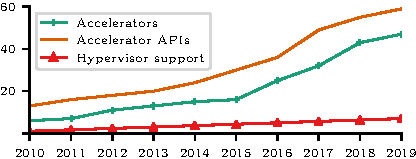
\includegraphics[width=0.7\linewidth]{ava/data/technology_trend/technology_trend.pdf}%
	\caption{The number of accelerators (discrete GPUs and AI
      accelerators) and APIs released since 2010 compared to the number of accelerators officially supported by production hypervisors (VMware ESX, Citrix XenServer, and Microsoft Hyper-V).
      % \ref{l:api_revisions} API major revisions; \ref{l:accelerator_arch} accelerator architectures; \ref{l:hypervisor_arch_support} accelerator architectures supported by hypervisors.
      This data was drawn from release notes and specification sheets.
      % TODO: \amp{This figure has been squished vertically. Regenerate with new aspect-ratio so as to avoid ugly squished text.}
  %\reviewer{F}{I don't think Fig 1 is of much use, your work is a case in point: A single automated approach can deal with many architectures and API revisions, so what is to be read from this?}
  %\cjr{F is pointing out our contribution, but somehow missing it. Dispatched by adding a bullet to the contribution list that claims exactly this.}
  }
	\label{fig:trends}
\end{figure}

Hypervisors have not kept pace with accelerator innovation. Figure~\ref{
fig:trends} shows the evolution of accelerator framework APIs, accelerator
architectures, and hypervisor support for them over the last decade.
Specialized hardware and frameworks emerge far faster than hypervisors support
them and the gap is widening. Many factors contribute to this trend, but lack
of demand is \emph{not} among them, evinced by the wide variety of
accelerators currently available from cloud providers~\cite{amazon_ec2,
google-gpu,google-cmle,gpucloud,amazon_f1,olympus,cloud-tpu}.
The challenge is technical: hypervisor-level accelerator virtualization
requires substantial engineering effort and the design space features multiple
fundamental trade-offs for which a ``sweet spot'' has remained elusive.

Practical virtualization must support sharing and isolation under flexible
policy with minimal overhead. The structure of current accelerator stacks
makes this combination extremely difficult to achieve.
Accelerator stacks are \emph{silos} (Figure~\ref{fig:silo}) comprising
proprietary layers communicating through memory mapped interfaces.
This opaque organization makes it \emph{impractical} to interpose intermediate
layers to form an efficient and compatible virtualization boundary
(\S\ref{s:properties}).
The remaining interposable interfaces leave designers with untenable
alternatives that sacrifice critical virtualization properties such as
interposition and compatibility.

This chapter describes \AvA, which addresses the fundamental limitations of
existing accelerator virtualization techniques.
\AvA combines API-agnostic para-virtual stack components with a DSL
(Domain-Specific Language) and a compiler to automate construction and
deployment of guest libraries, hypervisor-level resource management, and
\workers. \AvA uses an abstract para-virtual device to serve as a transport
endpoint for forwarding the public APIs of vendor-provided frameworks
(e.g. CUDA or TensorFlow). Unlike currently popular user-space API remoting
solutions~\cite{bitfusion,xaas,vmCUDA,rCUDA,cu2rcu}, \AvA preserves hypervisor-level resource management and strong isolation using a novel
technique called \emph{\hirafull (\hira)}.
\hira forwards API calls over hypervisor-managed communication
channels, inserting au\-to\-ma\-tically-generated resource management
components at the transport layer to enforce policies from the DSL
specification. Critically, \emph{automation} from \AvA enables hypervisors
to keep up with fast accelerator evolution: automatic generation of components
dramatically shortens the development cycle. As Figure~\ref{fig:trends}
suggests, a solution that tracks API framework evolution can track hardware
evolution as well.

\AvA supports a broad range of currently-shipping compute offload
accelerators. We virtualized \numaccelerators accelerators including NVIDIA
and AMD GPUs, Google TPUs, and Intel QuickAssist. Virtualizing an API
framework using \AvA requires modest developer effort: a single developer
virtualized OpenCL in a handful of days, a stark contrast to the person-years
of developer effort for VMware's SVGA II~\cite{dowty2009gpu} or BitFusion's
FlexDirect~\cite{bitfusion}. \AvA provides near-native performance
(e.g., 2.4\% slowdown for TensorFlow and 5.6\% for CUDA), enforces isolation
and fair sharing (\S\ref{s:properties}) across guests, and supports live
migration. \AvA is available on GitHub \mbox{\href{https://github.com/utcs-scea/ava}{utcs-scea/ava}}.

% Concretely, this chapter makes the following contributions:

% \begin{itemize}[nosep,leftmargin=1em,labelwidth=*,align=left]
% \item We demonstrate feasibility of automatically constructed virtual accelerator support, using a single technique to support many architectures, APIs, versions, and policies.
% \item We introduce \hirafull (\hira) to enable
% hypervisor-enforced isolation and sharing policies unachievable with current
% SR-IOV and API remoting systems (\S\ref{s:motivation}).
% \item We describe a novel DSL, \Lapis, for describing API functions, resources, and policies to enable automatic construction of virtual stacks starting from native API header files.
% \item We evaluate \AvA on \numaccelerators accelerators showing low effort, strong properties, and good performance (\S\ref{s:eval}).
% \item We identify fundamental challenges in the accelerator virtualization design space (\S\ref{s:background}).
% \end{itemize}

% -*- fill-column: 85; -*-
%!TEX root = ../dissertation.tex
\section{Background}
\label{s:background}


Cloud providers currently support compute accelerators using PCIe pass-through, which dedicates the device exclusively to a single guest.
Despite evidence of accelerator under-utilization~\cite{underutilizingcloud,simultaneous_multikernel,improving_gpu,gpl,fiddle}, and abundant
research~\cite{simultaneous_multikernel,improving_gpu,gpl,fiddle,zhang2018g,yeh2017pagoda}, no practical alternative yet exists.
This section provides background to explain this trend and motivates \Model's design.

\subsection{Virtualization Properties}
\label{s:properties}

Virtualization is a huge area---see~\cite{bugnion_neih_tsafrir} for comprehensive treatment.
We focus on properties critical for accelerator virtualization: \emph{interposition}, \emph{compatibility}, and \emph{isolation}.

\paragraphbe{Interposition.}
Virtualization decouples a logical resource from a physical one
through an indirection layer, intercepting guest interactions with
a virtual resource and providing the requested functionality using
a combination of software and the underlying physical resource.
Thus, virtualization works by \emph{interposing}
an interface, and changing or adding to its behavior.
Interposition is fundamental to virtualization and provides well-known benefits~\cite{waldspurger-iovirt}.
The choice of interface and the mechanism for interposing it
profoundly impacts the resulting system's practicality.
\emph{Inefficient} interposition of an interface (e.g. trapping frequent MMIO access) undermines
performance~\cite{suzuki2014gpuvm,yufull}; \emph{incomplete} interposition
compromises the hypervisor's ability to enforce isolation.
%If an interposed interface does not completely encapsulate the underlying resource,
%isolation may be lost.~\cjr{maybe ditch that last one.}

\paragraphbe{Compatibility} captures multiple related dimensions, including
robustness to evolution of interposed interfaces and adjacent stack layers,
and applicability across multiple platforms or related devices.
For example, full virtualization of a accelerators's hardware interface (\S\ref{s:bg_tech})
has \emph{poor} compatibility in that it works only with that device.
However, it has \emph{good} compatibility with guest software,
% (Table~\ref{tab:virt-comp}),
which will work without modification.
%, assuming the operating system has
%appropriate drivers for the device.
Current accelerator virtualization techniques
reflect a compromise between these two forms of compatibility.
%\Model gives up
%guest software compatibility, but compensates for that loss with automation (\S\ref{s:compiler}) to quickly
%adapt to software and hardware evolution (\S\ref{s:design}).


\paragraphbe{Isolation.} Cross-VM isolation is a critical requirement for
multi-tenancy:
when a resource is multiplexed among mutually distrustful tenants,
tenants must not be able to see/alter each other's data (\emph{data isolation}),
or adversely affect each other's performance (\emph{performance isolation}).
A poor choice of interposition mechanism and/or interface limits the system's ability to provide these guarantees: e.g., API remoting~\cite{bitfusion, rCUDA, mps}
%\amp{``often''?}
%\cjr{always}
%forwards interposed API calls from VMs to a shared remote server,
can have poor isolation (\S\ref{s:bg_api_remoting}) because the hypervisor is bypassed.
%Using separate servers for each protection provides isolation.

\begin{figure}[!t]
	\centering
	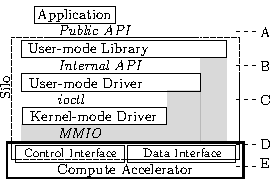
\includegraphics[width=.78\linewidth]{ava/images/silo.pdf}
	\caption{An accelerator silo.
		The public API and the interfaces with striped backgrounds are interposition candidates.
		All interfaces with backgrounds are proprietary and subject to change.
        %\cjr{Ref \S\ref{s:bg_tech} here?}\amp{Arrows removed to match more traditional idea of stack diagram and simplify drawing. Someone please second this choice.}
        %\cjr{seconded. Thanks!}
        }
	\label{fig:silo}
\end{figure}

\subsection{Accelerator Silos}
\label{s:silo}

% Accelerator vendors develop commodity software stacks
% using a common set of techniques.
Accelerator stacks
compose layered components that include a user-mode library to support an
API framework and a driver to manage the device.
Vendors are incentived to use proprietary interfaces and protocols between layers to preserve forward compatibility,
and to use kernel-bypass communication techniques to eliminate OS overheads.
However, interposing opaque, frequently-changing interfaces communicating with memory
mapped command rings is \emph{impractical} because it requires inefficient techniques and
yields solutions that sacrifice compatibility.
Consequently, accelerator stacks are effectively \emph{silos}
(Figure~\ref{fig:silo}), whose intermediate layers
\emph{cannot be practically separated} to virtualize the device.

\paragraphbe{Current support.} Most current hardware
accelerators feature some hardware support for virtualization: primarily for process-level
address-space separation, and in a small handful of cases, SR-IOV (\S\ref{s:bg_tech}).
A central premise of this paper is that hardware support for process-level isolation \emph{could}
suffice to support hypervisor-level virtualization as well, but the siloed structure of current accelerator stacks prevents it.

\begin{comment}
\begin{figure}[!t]
	\centering
  \vspace{-0.5em}
	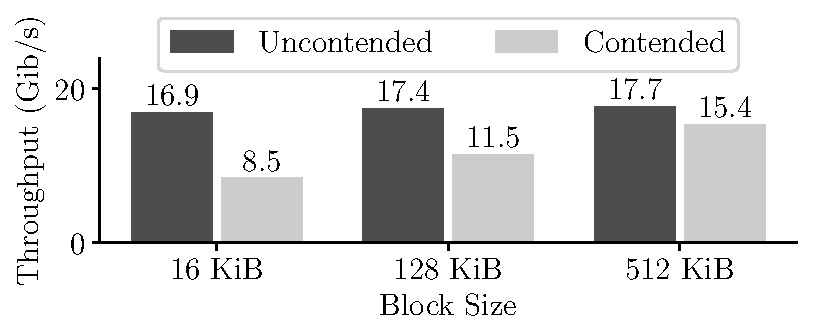
\includegraphics[width=.75\linewidth]{ava/data/rate_limit/qat_unfairness.pdf}
    \vspace{-.2cm}
	\caption{Throughput achieved by three instances of QATzip (running in VMs with SR-IOV pass-through) with different block sizes, running separately (\textbf{\texttt{Uncontended}}) and concurrently (\textbf{\texttt{Contended}}). Slowdown during concurrent execution is dependent on block size, i.e., the QAT HW scheduler cannot guarantee fairness.}
	\label{fig:qat-unfairness}
\end{figure}
\end{comment}

\subsection{Existing Accelerator Virtualization Techniques}
\label{s:bg_tech}


%% !TeX root = ../main.tex
\begingroup % Prevent leakage of length settings and defs into other files.

\def\chk{\checkmark}

\begin{table}[]
\resizebox{\columnwidth}{!}{%
\begin{tabular}{c|c|c|c|}
\cline{2-4}
                                      & isolated & interposition & compatibility \\ \hline
\multicolumn{1}{|l|}{PCIe PT}         &          &               &               \\ \hline
\multicolumn{1}{|l|}{FV}              & \chk     & \chk          &               \\ \hline
\multicolumn{1}{|l|}{MPT}             & \chk     &               &               \\ \hline
\multicolumn{1}{|l|}{PV}              & \chk     & \chk          &               \\ \hline
\multicolumn{1}{|l|}{SR-IOV}          & \chk     &               & \chk          \\ \hline
\multicolumn{1}{|l|}{API-Remote}      &          &               &               \\ \hline
\multicolumn{1}{|l|}{HIRA}            & \chk     & \chk          &               \\ \hline
\multicolumn{1}{|l|}{Automation+HIRA} & \chk     & \chk          & \chk          \\ \hline
\end{tabular}
}
\caption{
	Properties of virtualization techniques.
}
\label{tab:tech_compare}
\end{table}
%\hyu{Table~\ref{tab:tech_compare}}

%%% For accelerators, conventional virtualization techniques can be broadly classified according
%%% to which interface(s) they interpose (see Figure~\ref{fig:silo}) and which techniques are used to synthesize the
%%% virtual functionality.

\paragraphbe{PCIe pass-through}
is the current \emph{de facto} standard technique for exposing an accelerator to guest VMs.
It works by dedicating the hardware interface directly to the guest. Consequently,
it does not interpose \emph{any} interface. All benefits of virtualization are lost,
but native performance is preserved.

\paragraphbe{Full virtualization (FV)}~\cite{kvmgt,suzuki2014gpuvm,gVirt} interposes the hardware interface
(D in Figure~\ref{fig:silo}). For accelerators, this interface is memory mapped I/O (MMIO),
necessitating trap-based interposition (e.g. using memory protection or deprivileging), which
devastates performance (e.g., 100$\times$ or more~\cite{suzuki2014gpuvm, yufull}).
Accelerator hardware interfaces are proprietary and device-specific, so FV has poor compatibility,
even across different devices of the same type (e.g. AMD vs NVIDIA GPUs).
%Further full virtualization solutions rely on reverse-engineering of proprietary control interfaces, rendering them extremely tedious to build, maintain and evolve.

\paragraphbe{Mediated pass-through (MPT)} is a hybrid of pass-through and full virtualization.
MPT~\cite{gVirt,mdev-mvme,vpio}
uses pass-through for data plane operations, and provides a privileged
control plane interface for sensitive operations (D in Figure~\ref{fig:silo}).
MPT can preserve some of the raw speedup of
acceleration and allows guests to use native drivers and libraries.
However, limited interposition limits a hypervisor's ability to effectively manage resource sharing.
More importantly, hardware support is required and,
to our knowledge, Intel integrated GPUs are the only accelerators to support MPT~\cite{gVirt}.

\paragraphbe{Para-virtualization (PV)}
\emph{creates} an efficiently interposable interface in software and adjusts adjacent stack
layers to use it, rather than interposing an existing interface in the stack.
This necessitates a custom driver and library in every
supported guest OS for the virtual device.
The technique is powerful because enables encapsulation of diverse hardware
behind a single interposable interface.
However, compatibility is compromised: guest library and OS modifications are required,
and the para-virtual device interface must be maintained as interfaces evolve.
For example, VMware's SVGA II~\cite{svga} encapsulates
multiple GPU programming frameworks, but keeping up with the evolution of
those frameworks has proved untenable: SVGA remains multiple versions behind current frameworks~\cite{vmware_version,svga_guest} (e.g., DirectX~12~\cite{directx_version}).

\begin{comment}
\begin{figure}[!t]
	\centering
	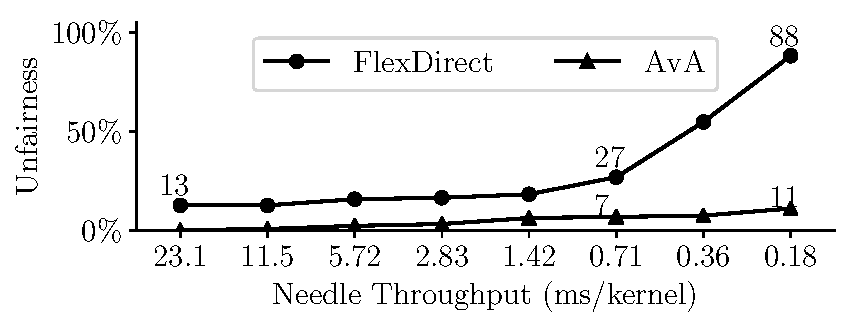
\includegraphics[width=.8\linewidth]{ava/data/rate_limit/bf_unfairness.pdf}
	\caption{Unfairness in slowdown between \lstinline|needle| and \lstinline|hotspot| applications in separate VMs running GPU kernels iteratively
    with BitFusion FlexDirect and \model.
    % When running alone, \lstinline|hotspot| has throughput of 126.3~ms/kernel.
    Fairness is calculated by $\left|s_1-s_2\right| \mathbin{/} (s_1+s_2),$
    where $s_i$ is the slowdown of application $i$ when running concurrently.}
	\label{fig:bitfusion_unfairness}
\end{figure}
\end{comment}

\paragraphbe{SR-IOV.}
Accelerators with PCIe SR-IOV~\cite{sriov} present multiple virtual devices (VFs) to system software.
%and the \emph{hardware} shares physical resources among them.
SR-IOV provides an interface and protocol for managing VFs, but the device vendor must \emph{implement} any cross-VF sharing support (E in Figure~\ref{fig:silo}) \emph{in silicon}.
The technique can provide strong virtualization guarantees~\cite{dong2012high,dong2008sr}, but hardware-level resource management
is inflexible and unevolvable: current implementations are trivially vulnerable to fragmentation and unfairness pathologies that cannot be changed.
Moreover, evidence is scant that broad SR-IOV support will emerge for accelerators:
only two current GPUs support it~\cite{amdfirepro,nvidiagrid}, none of the TPUs we evaluate support it;
and SR-IOV \emph{interface} IP blocks from FPGA vendors (used by~\cite{vu2014enabling,zazo2015pcie,vfpgamanager,huang2009fpgavirt}) do not implement resource management.
We do not expect this to change any time soon:
SR-IOV requires significant engineering effort vendors are not incentivized to invest.

\begin{figure*}[!!thp!]
	\centering
    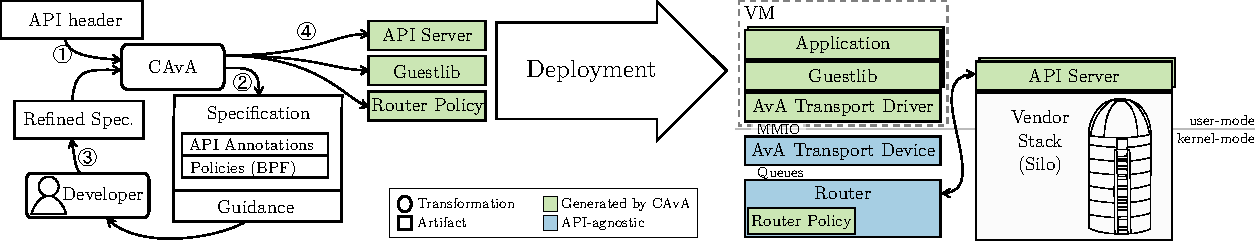
\includegraphics[width=\textwidth]{ava/images/overview.pdf}
    \caption{Overview of \model.
    %\hyu{The green and blue look the same when printed out.}
    %\amp{I don't see this problem. I increased contrast earlier today. check again?}
    %\hyu{Transport device is generated as well?}
    %\amp{Chris wanted it this way. The idea is to make the point that you need a new one for every API.}
    %\hyu{Color: it's better with my home printer but still hard to tell the difference from the legend. Device: then it conflicts with the text (\S4.1). I thought only the transport driver was generated for every API, but not the transport device.}
    %\cjr{this has converged.}
      %\amp{Tweaks if there is time: Remove extremely pale background on silo box. Separate colors more in brightness.}
    }
    \label{fig:overview}
    \vspace*{-1em}
\end{figure*}

\begin{comment}
\paragraphbe{Why is SR-IOV not the solution?} Full-featured SR-IOV from all accelerators is an unrealistic demand.
% Resource management must be baked into hardware;
Hardware designers tend to favor simple resource management policy implementations, easily leading to pathologies.
To illustrate the problem, we measured the throughput achieved by three VMs using Intel QuickAssist~\cite{QAT} (with SR-IOV) to compress data (offloaded with different chunk sizes), with and without contention (shown in Figure~\ref{fig:qat-unfairness}).
Each VM was assigned a PCIe Virtual Function (VF) exposed by the same Physical Function (PF), causing the hardware to schedule requests round-robin.
% The VMs offloaded compression in differing chunks ().
When there is no contention, each application achieves a similar throughput.
% ($\sim$17~Gib/s).
However, when the 3 applications were executed concurrently, the throughput achieved was a function of offload chunk size used, \emph{yielding unfairness that cannot be fixed without changing the hardware}.
%We argue that even if all accelerators were to provide SR-IOV, similar pathologies
%due to lost interposition and inflexible hardware-policy would be inevitable.
\end{comment}

\label{s:bg_api_remoting}
\label{s:bitfusion}
\paragraphbe{API Remoting}~\cite{gVirtuS,gupta2009gvim,VCL,duato2009efficient,li2011gpu,GridCuda,cu2rcu,xiao2012transparent,gupta2011pegasus,vcorfu}
interposes the top of the stack, between application and framework library (A in Figure~\ref{fig:silo}).
Similar to system call interposition~\cite{paradice, nooks, rio, vrio},
API calls are intercepted and forwarded to a user-level API framework~\cite{vCUDA} in an appliance VM~\cite{vmCUDA}, or remote server~\cite{rCUDA,kim2012snucl}.
Limited interposition frequency, batching opportunities~\cite{rCUDA} and high-speed networks~\cite{deplyrcuda, bitfusion} reduce overheads,
making it appealing to industry.
Dell XaaS~\cite{xaas}, BitFusion FlexDirect~\cite{bitfusion}, and Google Cloud TPUs~\cite{cloud-tpu} use it to support GPUs, FPGAs, and TPUs.
However, API remoting compromises compatibility if multiple APIs or API versions must be supported. Moreover the technique bypasses the hypervisor,
giving up the interposition required for hypervisor-enforced resource management.
Our experiments with commercial systems like BitFusion FlexDirect~\cite{bitfusion} show vulnerability to massive
unfairness pathologies (up to 88.1\%) that \model's hypervisor-level enforcement avoids (\S\ref{s:eval_rate_limit}).
% Deferring enforcement to trusted \worker{}s is a tenable alternative, but which requires integration with hypervisor-level resource management.
% Current solutions do not support it, and the engineering effort required would be substantial.
% \cjr{Better address \worker as trusted resource manager alternative? I think it's an isomorphic solution: hypervisor-integration is what's required,
% and \model could generate that instead, yielding the same properties. }
 %, or in some cases cannot even guarantee isolation between guests~\cite{mps}.
%Existing accelerator API remoting systems have required significant developer effort:
%systems like Bitfusion FlexDirect~\cite{bitfusion}, and rCUDA~\cite{rCUDA} reflect multi-year system-building efforts.~\cjr{find some way of characterizing that effort?}
%\reviewer{A}{The paper should probably mention the similarities in API forwarding and syscall interpositions since there is a large body of work in virtualization at the syscall level.}
%\cjr{observed in definition above--we should add a bunch of cites of course still.}
\begin{comment}
To illustrate fundamental shortcomings of user-level API remoting,
we experiment with contending VMs using .
FlexDirect's lack of hypervisor interposition means it cannot enforce hypervisor policy, leading to the potential for unfairness, particularly when kernel switch is frequent.
Figure~\ref{fig:bitfusion_unfairness} shows the problem on an NVIDIA GTX 1080:
FlexDirect is unfair (up to 88.1\%) when running two applications with different
kernel run-lengths (126.3~ms/kernel vs 0.18~ms/kernel in the worst case).
In contrast, \Model retains hypervisor interposition, and guarantees fairness (\S\ref{s:eval_rate_limit}).
\end{comment}

%% -*- fill-column: 85; -*-
%!TEX root = ../dissertation.tex


\subsection{Motivation}
\label{s:motivation}

For accelerator silos, the \emph{only} stable and
efficiently interposable interface is the framework API, so
we focus on techniques to recover or compensate virtualization properties lost by
API remoting: interposition and compatibility.
Interposition can be recovered by using hypervisor-managed forwarding transport,
creating a central interface at which to enforce resource management policies.
\Model uses a novel technique called \emph{\noveltechnique (\novtechabbrv)} to achieve this.
\novtechabbrv presents guest VMs with an abstract virtual device with MMIO Base Address Registers (BAR), but this device is \emph{not a virtual accelerator}, but an endpoint that
routes communication through the hypervisor.

Using hypervisor-managed transport recovers interposition, but complicates compatibility and introduces engineering effort:
\novtechabbrv requires custom guest libraries, guest drivers, and API servers for each OS and API, and API-specific resource-management code in the hypervisor.
\model mitigates this with automated construction (\S\ref{s:api}).
Automatically generating code to implement \novtechabbrv components presents several challenges which
follow from the need to specify API semantics and policies for which
existing Interface Description Languages (IDLs)~\cite{Lamb1987,MSIDL} are not applicable.
\Model uses a new DSL called \speclang, a compiler called \compiler, and device-agnostic transport components to address these challenges.

% because semantic information %and resource management
%specifications required for virtualization are beyond the scope of existing IDLs.
%sharing policy specifications that are beyond the scope of IDLs.
%Designing efficient and flexible transport layers, and enforcing resource-sharing policies at the transport layer where semantic %information about the underlying device resources is not readily available are additional challenges.
% In subsequent sections, we show how

% -*- fill-column: 85; -*-
%!TEX root = ../dissertation.tex

\graphicspath{{images/}}

\section{Design}
\label{s:design}
\label{s:motivation}

For accelerator silos, the \emph{only} stable and
efficiently interposable interface is the framework API, so
we focus on techniques to recover or compensate virtualization properties lost by
API remoting: interposition and compatibility.
Interposition can be recovered by using hypervisor-managed forwarding transport,
creating an interface at which to enforce resource management policies.
\Model uses a novel technique called \emph{\noveltechnique (\novtechabbrv)} to achieve this.
\novtechabbrv presents guest VMs with an abstract virtual device with MMIO Base Address Registers (BARs), but this device is \emph{not a virtual accelerator}, but an endpoint that
routes communication through the hypervisor.

Using hypervisor-managed transport recovers interposition, but complicates compatibility and introduces engineering effort:
\novtechabbrv requires custom guest libraries, guest drivers, and API servers for each OS and API, and API-specific resource-management code in the hypervisor.
\model mitigates this by
automatically generating code to implement \novtechabbrv components (\S\ref{s:api}), which introduces the
need to specify API semantics and policies beyond the ability of existing Interface Description Languages (IDLs)~\cite{Lamb1987,MSIDL}.
%\Model uses a new DSL called \speclang, a compiler called \compiler, and device-agnostic transport components to address these challenges.

\Model targets \emph{compute offload} accelerator APIs,
such as OpenCL, CUDA, and TensorFlow, which control an accelerator explicitly
through data transfer and task creation interfaces.
\Model consists of API-agnostic para-virtual stack components to
implement transport and dispatch for API remoting,
API-specific components that interpose and execute the API functions,
and a compiler, \compiler, which generates the API-specific components from a
specification of the API.
The API specification is written in a new high-level specification language, \speclang.
Figure~\ref{fig:overview} shows the work-flow to support a new API with \model (\S\ref{sub:workflow}) and the \model stack.
The API-agnostic components may be deployed in the hypervisor or in an appliance VM to support type I and II hypervisors~\cite{Popek1974-xx}.

\subsection{\Model Components}
\label{sub:components}
% \hyu{Reference to Figure~\ref{fig:high_level_design}?}
Figure~\ref{fig:overview} provides an overview of the interaction
between the various components in a \model-generated design.

The \parname{guest library} is generated by \compiler from the \speclang
specification. It provides the same symbols as the vendor library for the
application to link against.
The guest library intercepts all API functions called by
guest applications, marshals function arguments and implicit
state, and forwards the call through the transport channel for
remote execution.

The \parname{guest driver} interacts with the \vdev exposed
to the VM and provides a transport channel endpoint in the VM.
% Each guest-driver manages a set of command queues that are used to forward API
% calls to the \worker via the router.
\Compiler generates a separate transport driver instance for each API framework.
%The instances are identical, but independent at runtime.
%\amp{Do we need to say this last part? It's pretty much what ``instance'' means.}
%\cjr{I agree. We don't.}
% A custom driver per API framework is necessary to preserve cross-framework isolation
% and guest OS interposition.
% \hyu{For the complete story, this is vAcc driver (for transport) + virtio driver (for mediation \& transport).}

The \parname{\vdev}
is an abstract device exposed to the
guest to forward API calls
between the guest and the \worker.
The \vdev exposes %MMIO BARs for control and
%registers~\cjr{do we actually use control registers? What for if so?}\hyu{Only 4 registers are being used: one stores vm\_id, one stores zero copy buffer's physical address, two are used to notify KVM that the guestdrv is installed. Two deprecated registers were used to notify KVM that an app is spawned.},
a command queue interface.
It is API-agnostic, and its purpose is to
provide an interposable interface for the hypervisor.

The \parname{router} is an API-agnostic extension to the hypervisor that
implements \model's interposition logic. The router performs security
checks and enforces scheduling policies on forwarded API calls according
to the \speclang specification.

The \parname{\worker} is an API-specific user-space process generated
by \compiler. It runs either in an appliance VM (with PCIe pass-through access to the physical device) or in the host
and executes forwarded calls on behalf of the guest application.
A given \Worker is dedicated to a single guest process, leveraging
process-level isolation when the hardware supports it to guarantee fault and device context isolation.
%The \worker is a trusted component---the router may rely on the \worker to
%provide semantic information that may be specific to a given API, e.g., the
%\worker may provide device resource accounting information to the router for
%resource management.

\begin{comment}
\cjr{I think we've made the point already, and we need the space.}
The router and the specialized transport that enables it distinguishes \model from API remoting and allows \model to support hypervisor level interposition.\amp{might be a strawman. Someone please check and rewrite.}
The router, the \worker, and vendor
device drivers are considered part of the Trusted Computing Base, while the
guest library and the guest \vdev driver are untrusted.

\cjr{Anyone: Add sentence saying exactly how these components are different from traditional API remoting?}
\end{comment}

\subsection{Developer Work-flow}
\label{sub:workflow}

\Model's API-agnostic components (\S\ref{sub:components}) must be implemented for each hypervisor, along with the guest drivers
needed for each supported guest OS. The development effort to build them
is amortized across all of the accelerators and framework APIs supported.
%% The guest driver is only implemented once, but the illusion of having a
%% separate driver per API framework (necessary for isolating API frameworks and
%% maintaining interposition in the guest OS) is maintained by automatically
%% generating driver registration code for each API framework.

\Model's API-specific components are generated from \speclang by \compiler to
plug into \model's API-agnostic components.
% \Model uses \speclang (\S\ref{s:api}), which is used to annotate the APIs and
% accelerator resources, to automate the construction of the API remoting system
% for \emph{any} accelerator API.
% \reviewer{A}{How automated is the process if the programmer must annotate the API? What happens if the API changes?}
Figure~\ref{fig:overview} shows the work-flow to support a new API with \model.
First, \compiler automatically generates a preliminary \speclang specification from the unmodified header file.
% \cjr{Do we assert that the preliminary spec is correct but unoptimized? If not, how do we ensure the user deals with every missing element/problem area?}
% \hyu{Addressed by AMP in CAvA section.}
The programmer refines the specification with guidance from \compiler; adding information missing from the header file, e.g., buffer sizes or implicitly referenced state.
% , providing only the information that \compiler cannot infer.
Once the developer is satisfied with the API specification, she invokes
\compiler to generate code for the API-specific components and the customized
driver. \Compiler also generates deployment scripts.
% for compiling the generated code, and for integrating it with the API-agnostic components.
When a new version of an API is released, the same process can be used, starting with the previous specification.

% -*- fill-column: 85; -*-
%!TEX root = ../dissertation.tex

\graphicspath{{images/}}

\subsection{Communication Transport}
\label{s:design_transport}

\Model relies on an abstract communication channel that defines how
calls, and their associated data buffers, and results are sent, validated, and received.
%The channel interface provides primitives to send/receive commands.
% to marshal/unmarshal function arguments and  AMP: Our channel does not provide marshalling other than buffer attachment, so I don't think it's important and could confuse people as marshalling can imply things like encoding strings or numbers.
The channel provides an interposition point to track resources and invoke policies from the \speclang specification.
Using an abstract interface allows hypervisor developers to choose the best available communication transport
(e.g., shared memory FIFOs vs RDMA).
While the channel explicitly requires that all communication between the guest
and the \worker must take place through the router, no assumptions are made
about the actual location of components, which may be
disaggregated.


% \subsection{Callbacks}
%\label{s:callback}
\Model communication is bidirectional: it must support function callbacks from the \worker to the guest library, because
callbacks are fundamental in many frameworks, e.g., TensorFlow,
and must be run in the guest VM. % (instead of the \worker) to
%protect host domain from malicious code.\cjr{I think it would also be incorrect to run them anywhere else.}
In \model, the transport handles two types of payloads: \emph{commands} which contain opaque arguments and metadata for calls (e.g., thread ID and function ID) and \emph{data} which contains buffers referenced from the arguments (e.g., bulk data).

\subsection{Sharing and Protection}
\label{s:protection}

\Model re-purposes process-level isolation mechanisms (e.g. memory protection)
provided by the accelerator silo when it is available to simplify supporting cross-guest
isolation. We anticipate that emerging accelerators will support process-level isolation, as all GPUs do today.
% We reiterate that lack of hardware virtualization support is not the obstacle for accelerator virtualization,
% but stack structure is: if and when all accelerators support process-level virtualization in hardware,
% \model will still be necessary because vendor stacks do not expose the interfaces required to take advantage
% of that support.
%~\cjr{This last sentence is important, but too long.}
%~\cjr{But, we're going to keep it.}
For accelerators that do not natively support process-level isolation,
\model can still share device, relying on semantic information from additional \speclang descriptors
to generate code that supports coarse-grain time-sharing, leveraging the same state capture techniques we use for VM migration (\S\ref{s:migration}).
% A descriptor on functions that create and destroy connections to hardware allows
% the \compiler to insert additional logic in the device open/close calls to
% transparently spin until the device becomes available.
This solution admits no concurrency between tenants, but enables protected
sharing for devices which cannot otherwise be shared.

\subsection{Scheduling and Resource Allocation}
\label{s:rate_limit}
\label{s:api_throttling}

\Model can enforce policies (e.g., rate limiting) on shared resources,
e.g., device execution time, by tracking resource consumption and invoking
policy callbacks that change how API calls from
guests (\S\ref{sub:scheduling}) are scheduled.
The developer provides policy callbacks in the \speclang specification, and uses descriptors to identify how resources are consumed.
% ~\cjr{I assume this is a callback or something? The spec can't provide an approximation, but it can provide a way to get it, right?} of
%of the shared resource.
When such a descriptor is unavailable, \model falls back to coarse-grained
estimation of resource utilization, for example, using wall-clock time to approximate device execution time.
%We expect even such a rough approximation to be sufficient for useful policy enforcement.
% \hyu{We should say we can do better than wall-clock approximation.}
% \Model uses adaptive call rate limiting, based on proportional time-sharing
% and feedback control~\cite{scheduling_survey} (see \S~\ref{sub:scheduling}).

% The \model router schedules only API function calls, like previous API
% remoting systems. However, unlike previous systems, the router runs in the
% hypervisor, and can be integrated/federated with schedulers for other resources to
% improve locality and performance.

\subsection{Memory Management}

To support memory sharing on devices with onboard memory, \speclang resource usage descriptors
enable generated code to track the device memory
allocated to each guest VM. %based on the resource usage description in \speclang. In this scenario, the router would rely on the
%\worker to notify it of all allocation and deallocation of device memory.
Resource accounting code is auto-generated from semantic knowledge of
the device memory allocation APIs (such as, memory types and how to compute size
of buffer) provided by descriptors in the API specification.
%If a device memory allocation request would exceed the guest's quota,
%the \worker returns the appropriate Out-of-Memory (OOM) error for the allocation.

%\beginchanged
% -*- fill-column: 85; -*-
%!TEX root = ../dissertation.tex

\begingroup % A group to prevent \txt from leaking into following files.
\newcommand{\txt}[1]{\textrm{\it #1}}
\newcommand{\halfvspace}{} % \vspace*{0.25em}
\newcommand{\halfhspace}{\hspace*{0.25em}}
\newcommand{\spec}{\lstinline[language=C,style=nwspecc,columns=fullflexible]}

\graphicspath{{images/}}

\section{\CAvA and \Lapis}
\label{s:api}
\label{s:compiler}

The \AvA toolchain
comprises a language (\Lapis), a compiler (\CAvA), and a runtime library.
% AMP: The runtime is not written in Lapis. (It will be in Lapis 2, which I may well have mentioned at some point)
\CAvA accepts code written in \Lapis (\textbf{L}ow-level \textbf{API} \textbf{S}pecification), and generates C
source for an API-specific remoting stack that implements the \hira design.
\Lapis extends C declarations with descriptors to express a broad range of semantic information
necessary to generate that stack.
This includes information captured by traditional IDLs (e.g., function parameter semantics and data layout),
as well as information required for accelerator virtualization that is not expressible in existing IDLs.
% \Lapis is not inherently specialized for accelerator API remoting--the additional semantics
% required for \AvA are expressed in terms of more general language-level primitives:
% however, to simplify discourse, we will focus only on features relevant to \AvA.

To understand how \AvA relates to other IDL-based API-remoting techniques,
it is useful to compare it to the Sun Network File System~\cite{Sandberg:1988}.
NFS supports remote access to the the file system using
an IDL to specify API semantics and a compiler to automate code generation. NFS and \AvA share a number of
key challenges. Both must marshal and transfer function calls and arguments, handle asynchrony,
refactor functionality and (potentially implicit) state across newly decoupled components. Both must
preserve the resource management and sharing support expected for a resource managed by system software.

However, key differences between \AvA and NFS arise around additional virtualization requirements and
limitations in the design space.
For example, virtualization requires that \AvA be able to capture of
sufficient API-level state to enable features like live VM migration.
Key techniques used by NFS to deal with implicit state and
resource management are impractical \AvA.
NFS mostly \emph{eliminates} implicit state by altering the API,
e.g. replacing functions using implicit seek pointers with stateless read/write functions and offset parameters.
To deal with resource management, sharing, and compatibility challenges,
NFS \emph{introduced} the VFS layer, providing
an application-transparent interposition point at which to centralize or delegate that functionality using code written
to run at that layer. \AvA cannot alter APIs, so it exposes language-level features for dealing with implicit state.
\AvA cannot introduce new abstraction layers due to vendor opacity and API diversity: so the
resource management and sharing policy are expressed at the language layer as well.

% \paragraphbe{OS interposition.} A significant challenge faced by NFS was lack of a well-defined
% OS-level API for the file system, which is necessary for preserving OS-level resource management of the file
% system and providing compatibility at a software layer that minimizes application level change. While \AvA
% has the same problem (there are no standard OS-level interfaces for accelerators), the NFS designers had
% the luxury of simply defining one: the VFS layer is introduced for precisely this purpose.

% \paragraphbe{Difficult-to-capture API semantics.} API prototypes in a native header file do not fully
% specify the semantics of that API for a number of reasons. Some of missing semantics are
% straightforward to provide with an IDL specification, e.g. \texttt{in/out} semantics for arguments are absent,
% type layout for serialization, and relationships among individual function arguments such as buffer pointers and sizes.
% Some missing semantics are more difficult to capture in an IDL, for example API functions may
% refer to or manipulate context that is carried across API calls, such as seek pointers for \texttt{read} and \texttt{write} calls,
% which presents a design challenge for how to factor such implicit state\amp{context?} across the client/server boundary.
% Unlike NFS, which had the luxury of simply changing APIs to minimize implicit state (e.g. by replacing seek position with
% explicit offset parameters, or piggy-backing generation numbers on client file handles), \AvA does not have the
% luxury of changing APIs. Moreover, \AvA must contend with a number of additional requirements not
% present in NFS: enabling \emph{hypervisor-level resource management} requires semantic knowledge the relationship between
% API calls and accelerator-level resource management (e.g. how much memory is allocated, what fraction of the compute
% cycles are dedicated to individual guests), semantic knowledge of API-level \emph{object lifetimes} to support
% features such as live migration, and the ability to express resource management \emph{policies} that can be enforced by the hypervisor.

% While extending an existing IDL would provide \AvA with necessary semantics to deal with
% basic parameter marshalling, we know of none that capture all the semantics required to enable
% state tracking for device-side objects, abilitiy to express complex implicit API state, and
% support for expressing and enforcing resource management polcies. Moreover, while the guest library
% and API servers generated by \CAvA are analogous to the stubs and skeletons created by an
% IDL compiler, \AvA requires a backend specialize to additionally generate device driver code, and
% policy hooks to run in the hypervisor. Consequently, we chose to design a new language and compiler that
% meets these needs.

% \cjr{Present CAvA and LAPIS as a development platform: runtime library support is a key element.}

% -*- fill-column: 85; -*-
%!TEX root = ../main.tex

\begin{figure}
%@@cuMemcpyHtoDAsync(CUdeviceptr dst, void *src,|\label{line:cuMemcpyHtoDAsync}|
%           size_t size, CUstream stream)@@ { 
%  async; success(CUDA_SUCCESS);
%  argument(src) { in;|\label{line:src-in}| buffer(size); lifetime_manual; }
%  register_buf(async_HtoD, stream, src, size); }
\begin{lstlisting}[language=C,style=nwspecc,columns=flexible,belowskip=-0.5em,aboveskip=-0.5em,mathescape,basicstyle={\scriptsize\ttfamily}]
continuous_rc device_memory;
instantaneous_rc kernel_invocations;|\label{line:declare_rc}|
policy("policy_kern.c");|\label{line:scheduler_code}|
struct fn_arg_info {
  // CUfunction type information, filled by other LAPIS code
  int fn_argc;
  char fn_arg_is_handle[64];
  size_t fn_arg_size[64];
};
declare_metadata(struct fn_arg_info);
buf_registry async_DtoH;
type(CUdeviceptr) { handle; }|\label{line:cudeviceptr-handle}|
@@cuMemAlloc(CUdeviceptr *pp, size_t size)@@ { 
  allocates_rc(device_memory, size);|\label{line:allocates_rc}|
  argument(pp) { out; element { obj_record; allocate; } } }
@@cuMemcpyDtoHAsync(void* dst, CUdeviceptr src,|\label{line:cuMemcpyDtoHAsync}| 
                    size_t size, CUstream stream)@@ {
  async; success(CUDA_SUCCESS);|\label{line:success}|
  argument(dst) { no_copy;|\label{line:dst-nocopy}| buffer(size); lifetime_manual; }
  register_buf(async_DtoH, stream, dst, size); }
@@cuLaunchKernel(CUfunction f,
    uint gridDimX, uint gridDimY, uint gridDimZ,
    uint blockDimX, uint blockDimY, uint blockDimZ,
    uint sharedMemBytes, CUstream hStream,
    void **kernelParams, void **extra)@@ {
  async; consumes_rc(kernel_invocation, 1);|\label{line:consume_rc}|
  argument(kernelParams) {
    in; buffer(metadata(f)->fn_argc);
    element {
      if (metadata(f)->fn_arg_is_handle[index]) {
        type_cast(CUdeviceptr*); buffer(1);
      } else {
        type_cast(void*); buffer(metadata(f)->fn_arg_size[index]);
      } } }
  argument(extra) { in; ... } }
@@cuStreamSynchronize(CUstream stream)@@ {
  contextual_argument void** bufs =|\label{line:sync-bufs-1}| get_bufs(async_DtoH, stream);|\label{line:sync-bufs-2}|
  argument(bufs) {
    in; buffer(get_n_bufs(async_DtoH, stream));
    element { 
      buffer(get_buf_size(async_DtoH, stream, index));
      out; deallocate; } } }|\label{line:dst-buf-out}|
\end{lstlisting}
% no_copy; buffer(get_async_free_buf_size(stream, index));
\caption{
An example \speclang description for the CUDA driver API.
Code elements in {\lapiskeywordstyle bold blue} are \speclang keywords, elements in {\lapisstdlibstyle italic green} are runtime library calls, 
elements in {\lapisprototypestyle gray} are function prototypes incorporated by \compiler from the original CUDA header file,
and the remaining code is programmer-provided \speclang.
The variable \spec|index| is a \speclang builtin which provides the index of the current element of a buffer.
The specification of the argument \spec|extra| to \spec|cuLaunchKernel| is complex due to alignment and padding, and is elided from this example for clarity. 
%The specification of \spec|extra| is overall very similar to the specification of \spec|kernelParams|.
The file \spec|policy_kern.c| is shown in Figure~\ref{fig:scheduler_example}.
}
\label{fig:lapis-values-example}
\label{fig:spec_example}
\vspace*{-0.5em}
\end{figure}


\subsection{\Lapis}

A developer writing a \Lapis specification must be concerned with
capturing and expressing API semantics that fall roughly into four categories:
argument and data marshalling, asynchrony, explicit and implicit state,
and resource management policy.
To illustrate how \CAvA, \Lapis, and the runtime library,
work together to address these concerns, we will use a running example that
uses the CUDA driver API in an idiomatic scenario. The example allocates GPU memory (\texttt{cuMemAlloc}), makes
asynchronous calls using CUDA streams to transfer data before (\texttt{cuMemcpyHtoDAsync}) and after (\texttt{cuMemcpyDtoHAsync}) launching a kernel (\texttt{cuLaunch\-Kernel}),
and synchronizes the stream (\texttt{cuSynchronize\-Stream}).
The \Lapis source for the four of the five CUDA API functions required is shown in \autoref{fig:lapis-values-example}. We
elide source for \texttt{cuMemcpyHtoDAsync} because it is conceptually similar to \texttt{cuMemcpyDtoHAsync}.

\Lapis extends C types and function prototypes with information to serialize arguments and return values,
and manage user-defined metadata on API-level objects such as GPU kernels or memory buffers. The latter can be used to
specify the higher-level semantics and behaviors required for virtualization such as how to capture, transfer, and synchronize implicit state.
Descriptors are embedded in \Lapis function declarations,
can be flexibly scoped (\autoref{tab:lapis-scope}), and
applied to values (\autoref{tab:lapis-values}) or functions (\autoref{tab:lapis-functions}).
%A descriptor can also use a \Lapis keyword to apply to an \spec|argument|, an \spec|element| of a buffer, or all instances of a \spec|type|.
Descriptors can be conditional using an \spec|if| statement.
In the following discussion of \Lapis descriptors, we use the term ``this function'' to refer the function
being described or the function whose argument is being described.

\paragraphbe{Marshalling and Managing Values and Objects.}
\Lapis value descriptor usage is illustrated by the CUDA function \spec|cuMemcpyDtoHAsync| defined in \autoref{fig:lapis-values-example} (Line~\ref{line:cuMemcpyDtoHAsync}).
The argument \spec|src| is only used by the application through API calls
(\AvA does not currently support UVM, see \S\ref{s:limitations} for details).
This is true of the type \spec|CUdeviceptr| in general, so it
is expressed on line~\ref{line:cudeviceptr-handle} with \spec|type(CUdeviceptr) { handle; }|.
The \spec|handle| descriptor enables \AvA to generate code that implements an indirection layer for accessing it.
The argument \spec|dst| is a pointer to an application buffer of length \spec|size|; this is expressed on line~\ref{line:dst-nocopy} with \spec|argument(dst) { no_copy;| \spec|buffer(size); }| which selects the argument \spec|src| and specifies it as a \spec|buffer| of \spec|size| length.
The buffer will be copied back to the application later so it is \spec|no_copy| here.
Because the function is asynchronous (see below), the buffer for \spec|src| in the \worker must exist at least until the copy has completed:
the descriptor \spec|lifetime_manual| on line~\ref{line:dst-nocopy} states that the specification will indicate when the buffer is no longer needed using \spec|deallocate| (line~\ref{line:dst-buf-out}).
%On line \ref{line:src-in} \spec|in| informs \CAvA that the buffer will only be read by the call and should be copied from the application to the \worker before the call.
%The argument \spec|size| is a primitive value so \CAvA can simply copy its value directly from the application to the \worker. This is the default, so no descriptor is needed.
%The \spec|cuMemcpyDtoH| specification is similar except the types of \spec|src| and \spec|dst| are switched and the buffer argument is now annotated with \spec|out| since it will be written by the call and needs to be copied back to the application thereafter.

% -*- fill-column: 85; -*-
%!TEX root = ../main.tex

% NOTE: TexLive 2017 fails when a lstlisting environment is inside a table. This is fixed in 2018, but
% multirow still has the issue. Because of this, I'm using saveboxes for a bunch of listings just in case.
\newsavebox{\boxargumentsyntax}
\begin{lrbox}{\boxargumentsyntax}
\begin{lstlisting}[language=C,style=nwspecc,columns=fullflexible,numbers=none]
argument(x) {
  descriptors }
\end{lstlisting}
\end{lrbox}

\newsavebox{\boxelementsyntax}
\begin{lrbox}{\boxelementsyntax}
\begin{lstlisting}[language=C,style=nwspecc,columns=fullflexible,numbers=none]
element {
  descriptors }
\end{lstlisting}
\end{lrbox}

\newsavebox{\boxtypesyntax}
\begin{lrbox}{\boxtypesyntax}
\begin{lstlisting}[language=C,style=nwspecc,columns=fullflexible,numbers=none]
type(ty) {
  descriptors }
\end{lstlisting}
\end{lrbox}

\newsavebox{\boxifsyntax}
\begin{lrbox}{\boxifsyntax}
\begin{lstlisting}[language=C,style=nwspecc,columns=fullflexible,numbers=none]
if (pred) { 
  descriptors1
} else {
  descriptors2 }
\end{lstlisting}
\end{lrbox}

\begin{table}
  \centering
\resizebox{\columnwidth}{!}{
  \begin{tabular}{@{}p{1in} p{3in}@{}}
  \toprule
  Scope & \spec|descriptors| in this scope apply to ...  \\
  \midrule 
  \raisebox{-0.5em}{\usebox{\boxargumentsyntax}}  & the argument \spec|x|, called the described argument. \\
  \raisebox{-0.5em}{\usebox{\boxelementsyntax}} & the referenced value, called the described value; e.g., if applied to an argument \spec|x|, the descriptors inside apply to \spec|*x|. \\
  \raisebox{-0.5em}{\usebox{\boxtypesyntax}} & all values of type \spec|ty|. \\
  \raisebox{-1.7em}{\usebox{\boxifsyntax}} & \spec|descriptors1| apply only if \spec|pred| is true; \spec|descriptors2| apply otherwise. \\
  \bottomrule
  \end{tabular}
  }
  \caption{\speclang syntax which values descriptors apply to and when those descriptors apply.
  %\cjr{maybe we can refactor this   whole thing into the sentence that says descriptors are flexibly scoped.}
  }
  \label{tab:lapis-scope}
%  \vspace*{-1em}
\end{table}

% -*- fill-column: 85; -*-
%!TEX root = ../main.tex

\begin{table}
  \centering
\resizebox{\columnwidth}{!}{
  \begin{tabular}{@{}p{1in} p{3in}@{}}
  \toprule
  Type & The value is ... \\
  \midrule
  \spec|type_cast(ty)| & type \spec|ty| and should be cast in the generated code. \\
  \spec|handle| & an API object handle. \\
  \spec|buffer(size)| & a buffer of \spec|size| elements. \\
%  \spec|zerocopy| & an \AvA zero-copy buffer allocated using \spec|zerocopy_alloc|. \\
  \spec|in| & an input and should be copied from the application to the \worker before the call. \\
  \spec|out| & an output and should be copied from the \worker to the application after the call. \\
  \spec|no_copy| & a buffer which should not be copied. Useful when combined with lifetimes. \\
  \spec|lifetime_call| & a buffer which need only exist in the \worker for the length of the call. (default) \\
  \spec|lifetime_manual| & a buffer which should exist in the \worker until it is explicitly deallocated. \\
  \spec|allocate| & a buffer which calls to this function allocate. \\
  \spec|deallocate| & a buffer which calls to this function deallocate. \\
  \spec|zerocopy| & a buffer which should be in zero-copy memory. \\
  \midrule
  \end{tabular}
  }
\resizebox{\columnwidth}{!}{
  \begin{tabular}{@{}p{1in} p{3in}@{}}
  \multicolumn{2}{@{}l}{API Object Recording}\\
  \midrule
  \spec|obj_record| & This call should be recorded and associated with the described value. The recorded calls capture the implicit state of the value. \\
  \spec|obj_depends_on(obj)| & Add a dependency between the described value and \lstinline|obj|, enabling \lstinline|obj| to be recreated if the described value is needed. \\
%  \amp{This really is it. This has no sync implications, since playback is sequential. This is actually almost always inferred, we could actually leave it out of the paper pretty safely.}
  \spec|obj_state_cbs(write, read)| & Attach state serialization and deserialization (\spec|write| and \spec|read|, resp.) functions to the described value. The serialized data captures the explicit state of the value and may be used in combination with implicit state. \\
  \bottomrule
  \end{tabular}
  }
  \caption{\Lapis descriptors for specifying values and objects.}
  \label{tab:lapis-values}
%  \vspace*{-1em}
\end{table}


\paragraphbe{Asynchrony and Implicit State.} \Lapis supports descriptors
for expressing semantics that arise due to asynchrony.
Most commonly, these are expressed by applying descriptors to functions.
For example, \spec|cuMemcpyDtoHAsync| in \autoref{fig:lapis-values-example}
is asynchronous and can return \spec|CUDA_SUCCESS| before the copy completes;
this is expressed using \spec|async| and \spec|success| on line~\ref{line:success}.
%The function descriptors in \autoref{tab:lapis-functions} specify function-level metadata,
%such as kernel parameter types or other special processing needed to make a remote call.
%The \spec|sync| and \spec|async| descriptors specify if a call from the application can return immediately while \AvA handles the call asynchronously, e.g. to improve performance.
% by overlapping \worker and application-level work.
%Asynchronous functions return a value to the application as specified by the \spec|success| descriptor (line~\ref{line:success}).
%Forwarded API calls may need to copy buffers which are not explicitly exposed as arguments to the API function.
%For example,
%because the \worker maintains shadow copies of buffers,
Asynchrony can also create implicit API-level state whose semantics must be expressed.
\spec|cuStreamSynchronize| must copy buffers back to the guest if there are outstanding asynchronous copies.
Those buffers may not be updated in the \worker until the call completes, so copy-back must be delayed to this point.
This requirement is expressed by passing dependent buffers using \spec|contextual_argument| along with the normal explicit arguments. The \Lapis code on line \ref{line:sync-bufs-1}--\ref{line:dst-buf-out}
uses this technique along with runtime library functions to track buffers dependent on ongoing asynchronous copies.
\AvA supports zero-copy transport of buffers: if a buffer allocation is described with \spec|zerocopy|, \CAvA allocates zero-copy memory for the application-side buffer.
%this is an important optimization for high-throughput APIs (e.g., kernel bypass APIs).
%The current implementation only supports this in a few specific cases, but this is not a fundamental restriction.

%\autoref{tab:lapis-functions} also includes descriptors for resource accounting and sharing policy.
%These are used in \autoref{fig:lapis-values-example}.
\paragraphbe{Resource Management and Policy.}
\Lapis supports descriptors to express the resources consumed by API functions.
Resources may be either \emph{instantaneous} or \emph{continuous}.
Instantaneous resources are consumed by an API function implementation only once,
e.g., by executing a GPU kernel upon request. Accounting works by measuring resources used at each function invocation.
In general, instantaneous resources are used to control throughput in some way; e.g.,
limiting the amount of compute resource a client is allowed to use in a fixed interval of time.
Continuous resources capture the ability an API implementation to assign a resource to a client for a
period of time. Accounting for continuous resources tracks resources assigned to each client/VM.
For example, GPU memory is a continuous resource limited by available physical memory,
which needs to be allocated
according to a sharing policy that manages cross-VM contention for it.

\autoref{fig:lapis-values-example} uses descriptors to track kernel calls (\spec|cuLaunch|\-\spec|Kernel|) and GPU memory allocation.
In \Lapis, this is expressed using two resources and descriptors on functions to specify how much of each resource is consumed.
Line~\ref{line:declare_rc} declares a resource representing function invocation rate.
Line~\ref{line:scheduler_code} specifies the custom policy used to schedule function invocations.
Line~\ref{line:consume_rc} specifies that a call to \spec|cuLaunchKernel| counts as one unit of the \spec|kernel_calls| instantaneous resource.
Line~\ref{line:allocates_rc} specifies that a call to \spec|cuMemAlloc| allocates \spec|size| bytes of the continuous resource \spec|gpu_mem|.


%For some instantaneous resources (e.g., data transfer over the bus), the amount can be estimated based on the arguments to a function call (buffer size).
%For other instantaneous resources (e.g., computation), the amount needs to be computed after the fact by measure how long the call or calls took to complete.
%Because of this, resource usage descriptors may be handled after a call completes by some Lapis compilers.

To specify policies, developers provide functions that schedule API calls from different VMs based on the recorded resource usage of those VMs. In our current implementation, policy functions are specified as eBPF programs stored in a separate file and referenced from the \Lapis source using \spec@policy("policy_kern.c")@ at the top level. In future work, we plan
to extend \Lapis to express these policies directly. We currently use eBPF because it enables unprivileged code to run
safely in the hypervisor and is available today, enabling \AvA to be used without modifying the hypervisor and without trusting the developer. However, in principle, the same properties can be achieved using \Lapis
and will provide a significant complexity reduction for the developer.
%However, the policy function could be run in privileged context if it were trusted, or could be run using any other technique for unprivileged execution inside the kernel.
%However, eBPF is already available, avoiding the requirement of additional changes to the kernel.

% -*- fill-column: 85; -*-
%!TEX root = ../main.tex

% NOTE: TexLive 2017 fails when a lstlisting environment is inside a table. This is fixed in 2018, but
% multirow still has the issue. Because of this, I'm using saveboxes for a bunch of listings just in case.
\newsavebox{\boxutilitysyntax}
\begin{lrbox}{\boxutilitysyntax}
\begin{lstlisting}[language=C,style=nwspecc,columns=fullflexible,numbers=none,belowskip=-2.2em,aboveskip=-1em,mathescape]
utility $\txt{C declaration}$;
\end{lstlisting}
\end{lrbox}

\begin{table}
  \centering
\resizebox{\columnwidth}{!}{
  \begin{tabular}{@{}p{1.31in}@{}p{2.7in}@{}}
  \toprule
  Function & The function ... \\
  \midrule
  \spec|sync| & is synchronous: application calls wait for completion in the \worker. \\
  \spec|async| & can be asynchronous: calls will return immediately after call dispatch. \\
  \spec|success(v)| & should return \spec|v| when called with \spec|async|. \\
  \spec|contextual_argument| & has additional context that should be transported along with the normal arguments. This is used to copy values or buffers which are not explicitly arguments to the call, e.g., \spec|errno|.
%  Contextual arguments can be annotated as usual.
  \\
  \spec|allocates_rc(r, x)| & allocates \spec|x| units of the continuous resource \spec|r|. \\
  \spec|deallocates_rc(r, x)| & deallocates \spec|x| units of the continuous resource \spec|r|. \\
  \spec|consumes_rc(r, x)| & consumes \spec|x| units of the instantaneous resource \spec|r| during the call. \\
  \midrule
  Declarations & The statement declares ... \\
  \midrule
  \spec|continuous_rc r;| & a continuous resource \spec|r|. \\
  \spec|instantaneous_rc r;| & an instantaneous resource \spec|r|. \\
  \usebox{\boxutilitysyntax} & a global utility function or variable that is not part of the API, but is used in the specification. \\
%  \usebox{\boxreplacesyntax} & a replacement for an API function that should be used within the guest application instead of forwarding the call to the \worker.  \\
  \bottomrule
  \end{tabular}
  }
  \caption{\Lapis descriptors for functions.
%  \amp{CJR, you have opinions on where these tables should be. Tell me what you want and I'll make it happen. I think the tables are close to stable.}
%  \amp{Use ``rc'' as a contraction for ``resource''?}\hyu{Make sure Figure 9 uses the same short form.}
  }
  \label{tab:lapis-functions}
\end{table}



\begin{table}
  \centering
\resizebox{\columnwidth}{!}{
  \begin{tabular}{@{}p{1.4in}@{}p{2.7in}@{}}
  \toprule
  Metadata &  \\
  \midrule
  \spec|declare_metadata(ty)| & Specify the type of value to store as metadata to be \spec|ty|.  \\
  \spec|metadata(key)| & Get, creating if needed, the metadata object associated with \spec|key|. \\
  \midrule
  In-flight buffers &  \\
  \midrule
  \spec|buf_registry r;| & Declare \spec|r| to be a registry of buffers. \\
  \spec|register_buf(r, k,|\newline\spec| buf, size)| & registers \spec|buf| which is \spec|size| elements attached to key \spec|k| (e.g., a CUDA stream) in registry \spec|r|. \\
  \spec|get_bufs(r, k)| & gets an array of the buffers attached to key \spec|k| in registry \spec|r|. \\
  \spec|get_n_bufs(r, k)| & gets the number of buffers return from \spec|get_bufs|. \\
  \spec|get_buf_size(r, k, i)| & gets the size of a specific registered buffer. \\
  \midrule
  Zero-copy &  \\
  \midrule
  \spec|zerocopy_alloc(n)| & Allocate \spec|n| bytes of zero-copy memory. \\
  % shared between the guest application and the \worker.
  \spec|zerocopy_free(p)| & Free the zero-copy memory pointed to by \spec|p|. \\
%  \spec|zerocopy_get_physical_address(p)| & Get the physical address of the zero-copy buffer \spec|p|. For use with APIs which require physical addresses for DMA (e.g., Intel QuickAssist). \\
%  \midrule
%  Misc. &  \\
%  \midrule
%  \spec|strlen(s)| & return the length of a \spec|NULL| terminated string. \\
%  \spec|min(x, y)|/\spec|max(x, y)| & return the minimum/maximum of two values. \\
  \bottomrule
  \end{tabular}
  }
  \vspace{.1cm}
  \caption{An except from the \Lapis standard library for use in expressions and utility functions.
%  \amp{Remove \spec|_type| from \spec|declare_metadata_type(ty)|?}
%  \hyu{Vote for \spec|declare_metadata(type)|.}\amp{\spec|type| is a keyword in Lapis as presented. So we cannot use it there without confusion.}
}
  \label{tab:lapis-stdlib}
\end{table}

\paragraphbe{State Capture.} To support VM migration, \AvA must capture the state of API objects and recreate that state at the destination. This requires visibility into the relationships between API calls
and device state: \AvA cannot simply serialize, transfer, and deserialize device state to
effect a migration because \AvA's view of device state is through the high level API and through
semantics specified by the programmer.
\AvA splits object state into two categories based on descriptors from the \AvA programmer.
\emph{Explicit} state is serialized into \AvA-managed storage by programmer-defined functions;
\emph{implicit} state is captured by recording calls which mutate an \emph{object} (e.g. a buffer) based on \spec|obj_record| descriptors. In \autoref{fig:lapis-values-example}, \spec|obj_record| descriptor is used in
\spec|cuMemAlloc| to expose implicit state, in this case a device-side buffer which must be allocated to recreate state at the destination.

\paragraphbe{Runtime Library.}
The \Lapis standard library is illustrated (in excerpted form) in \autoref{tab:lapis-stdlib},
and is designed to support common features we encountered across multiple APIs.
State tracking often requires storing metadata about an API object, so the library provides a system to do that.
Many APIs support asynchronous functions for which buffers tracking is required, so the library provides a set of function to track buffers.
For APIs that require zero-copy data transfer for performance or because they expose hardware doorbells, the library provides memory management functions that expose \AvA's support for zero-copy buffers.
%In addition to those listed, t
The library also provides common utilities
%which are common in the expression which commute the size of buffers,
such as \spec|min|, \spec|max|, and \spec|strlen|.

%\cjr{This should describe common utility functions as well as whatever built-in eBPF policies we already provide.}
%\amp{I would really prefer to keep the eBPF stuff separate. It cannot be used along with the Lapis utilities and cannot even appear in the same file.}
%\cjr{OK, that's fine. We should still add a very brief description of what's in the table of library APIs. Doesn't need to be long.}


%\AvA allows for zero-copy data transfer for buffers that are allocated via API function (e.g., \spec|cuHostMemAlloc|).
%However, the current implementation only supports the limited case where the API allocation functions can be replaced with \AvA specific implementations using the zero-copy allocation functions listed in \autoref{tab:lapis-stdlib}.
%An improved implementation could use the original API functions and then make those buffers available in the guest application.


% -*- fill-column: 85; -*-
%!TEX root = main.tex

\begin{figure}
\begin{lstlisting}[language=C,columns=flexible,mathescape,belowskip=0em,aboveskip=0em,basicstyle={\scriptsize\ttfamily}]
CUresult cuStreamSynchronize(CUstream stream) {
  // Allocate and initialize the command
  cu_stream_synchronize_call *cmd = $\txt{allocate}$;
  cmd->command_id = CALL_CU_STREAM_SYNCHRONIZE;
  cmd->call_id = generate_call_id(); // Unique call ID
  cmd->stream = stream;                    // Copy simple value
  // Compute and attach contextual parameter bufs
  void **bufs = get_bufs(async_DtoH, stream);
  size_t nbufs = get_n_bufs(async_DtoH, stream);
  // Attached buffers referenced from bufs
  void **tmp_bufs = $\txt{allocate and fill with output buffer sentinal}$;$\label{line:bufs-start}$
  cmd->bufs = attach_buffer(cmd, tmp_bufs, 
     get_n_bufs(async_DtoH, stream) *$$ sizeof(void *));$\label{line:bufs-end}$
  // Create and register a local record of the call
  cu_stream_synchronize_record *record = $\txt{alloc}$();
  record->stream = stream; record->bufs = bufs;
  record->call_complete = 0; register_call(record);
  // Send the command and wait for and return response
  send_command(cmd);
  wait_until(record->call_complete);
  return record->ret; }
CUresult cuMemcpyDtoHAsync(void *dst, CUdeviceptr src, 
                               size_t size, CUstream stream) {
  |\elidedcode{Allocate and initialize the command as above}|
  // Execute state-tracking code from spec
  register_buf(async_DtoH, stream, dst, size);
  |\elidedcode{Store and attach arguments similar to above}|
  |\elidedcode{Create and register a local record of the call, and send}|
  // Return the success value from LAPIS specification
  return CUDA_SUCCESS; }
\end{lstlisting}
\caption{An outline of the generated guestlib code for \spec|cuStreamSynchronize| and \spec|cuMemcpyDtoHAsync|. 
The real code manages a number of additional details, e.g., threads.
}
\label{fig:generated-code-outline-guest}
\vspace*{-0.5em}
\end{figure}


\paragraphbe{Workflow.}
In the \AvA workflow, \CAvA is initially invoked on the API header files to generate a provisional \Lapis specification for all functions in the API;
the developer then refines that specification.
For perspective,
the actual provisional specification generated by \CAvA for the functions in Figure~\ref{fig:spec_example} totals 107~lines,
of which 29~lines are deleted, 9~lines are changed, and 21~lines are added to reach the final specification used in our evaluation.
%Utilities called in these functions total 17~lines.
%\hyu{total (cuLaunchKernel 51, cuMemcpyHtoDAsync 25, cuMemAlloc 17, cuStreamSynchronize 14),
%deleted (13,6,5,5), changed (4,3,2,0), and added (9,6,0,6).
%(\lstinline|cuLaunchKernel_extra_size| 6, \lstinline|__helper_load_async_buffer_list| 11.)}
\CAvA can infer the semantics of functions and arguments in simple cases and provides safe defaults when possible (e.g., by default, functions are synchronous and numeric types are opaque).
For cases that do not admit a conservative guess, \CAvA emits code that will cause an error, e.g., for ``direction'' (in/out parameters),
which provides programmer guidance about what additional information is required and where it should be expressed.

Writing a \Lapis specification requires user-level knowledge of the API.
The developer must understand the API function semantics but does not need to know how to implement the API or understand details of \AvA or API remoting.
Our experience is that most APIs (e.g., OpenCL~\cite{opencl}) provide documentation sufficient to achieve this.
However one API (the CUDA runtime API)
required \Lapis specifications for undocumented functions which required more developer effort to produce. The real target users of \AvA
are hypervisor developers, cloud providers, and accelerator vendor software engineers, for whom the required knowledge can be safely assumed, and for whom
the reduction in development effort is compelling even for complex APIs.

\subsection{Code Generation}
\label{s:code_gen}

% \CAvA generates C source code from the API specification using templating.
% \CAvA builds simplified intermediate representation of the specification, \CAvA-IR.
% \CAvA-IR is similar to \Lapis, but it applies a fixed set of descriptors to every value (e.g., argument) and combines all conditionals into expressions which compute specification values (e.g., the boolean representing that a function is synchronous).\amp{Is this clear?}\cjr{DISCUSS}

\CAvA generates several separate components for each API function, including a stub function, a call handler, a return handler, and a replay handler for VM migration.
%The stub functions and return handlers are in the guest library, while call handlers are in the \worker, except in the case of callbacks, for which the placement is reversed.
%Replay handlers are always in the \worker.

% -*- fill-column: 85; -*-
%!TEX root = main.tex

\begin{figure}
\begin{lstlisting}[language=C,columns=flexible,belowskip=-0.5em,aboveskip=-0.5em,mathescape,basicstyle={\scriptsize\ttfamily}]
void api_server_handle_command(call) {
  switch (call->command_id) {
  case CALL_CU_STREAM_SYNCHRONIZE: {
    // For handles, get the real address
    CUstream stream = handle_deref(call->stream);
    // Get pointers to shadows of the attached buffers
    void **bufs = get_buffer(call, call->bufs);
    size_t nbufs = get_n_bufs(async_DtoH, stream);
    for (size_t i = 0; i < nbufs; i++)
      bufs[i] = get_shadow_buffer(call, bufs[i]);
    // Perform call
    CUresult stat = cuStreamSynchronize(stream);
    // Construct and send the return command
    cu_stream_synchronize_ret *ret_cmd = $\txt{alloc()}$;
    ret_cmd->command_id = RET_CU_STREAM_SYNCHRONIZE;
    ret_cmd->call_id = call->call_id; ret_cmd->ret = stat;
    // Attach sync buffers to return command
    void **tmp_bufs = $\txt{alloc()}$;$\label{line:sync-bufs-start}$
    for (size_t i = 0; i < nbufs; i++)
      tmp_bufs[i] = attach_buffer(ret_cmd, bufs[i],
         get_buf_size(async_DtoH, stream, i));
    ret_cmd->bufs = attach_buffer(ret_cmd, tmp_bufs, 
       nbufs *$$ sizeof(void *));$\label{line:sync-bufs-end}$
    send_command(ret_cmd);
    break; }
  case CALL_CU_MEMCPY_DTOH_ASYNC: {
    |\elidedcode{Extract dst, stream, and size from call}||\label{line:extract-start}|
    // Get or allocate the shadow buffer
    void *dst = get_shadow_buffer(call, call->dst);|\label{line:extract-end}|
    // Execute state-tracking code from spec
    register_buf(async_DtoH, stream, dst, size);|\label{line:register-buf}|
    // Perform call
    CUresult stat = cuMemcpyDtoHAsync(dst, src, size, stream);
    |\elidedcode{Construct and send the return command}|
    break; } ... } }
\end{lstlisting}
\caption{An outline of the generated \worker code for \spec|cuStreamSynchronize| and \spec|cuMemcpyDtoHAsync|.
}
\label{fig:generated-code-outline-worker}
\vspace*{-.5em}
\end{figure}


The generated stubs, in \autoref{fig:generated-code-outline-guest}, construct a command from the arguments (including handling lists of asynchronous output buffers on lines~\ref{line:bufs-start}--\ref{line:bufs-end}) and then send it, via the hypervisor, to the \worker.
The hypervisor enforces resource sharing policy at the router based on the resource accounting and policy descriptors.
The \worker, in \autoref{fig:generated-code-outline-worker}, deserializes the arguments from the command and then performs the real call.
The results of the call are passed back to the guest lib in the same was as the call is made.
The \worker also transfers (lines~\ref{line:sync-bufs-start}--\ref{line:sync-bufs-end}) the shadow buffers registered during calls to \spec|cuMemcpyDtoHAsync| (line~\ref{line:register-buf}) back to the guest.
The guest lib handles the response by completing record-and-replay tracking, looking up the API call record, copying transferred shadow buffers into application buffers, and marking the call complete (code elided for brevity).

% The guest lib handles the response as shown in \autoref{fig:generated-code-outline-guest-handle}.
%The \Lapis specification provides all the information needed for \CAvA to generate serialize and deserialize the arguments since the specification provides enough information to traverse all the argument data structures.
%\amp{The example generated code here is for a function not in the example spec. We should update this code to match some function in the spec.}
%As an example Figures \ref{fig:generated-code-outline-structs}--\ref{fig:generated-code-outline-worker} show an outline of code generated for \spec|cuMemcpyHtoD| from \autoref{fig:lapis-values-example}.
%
\begin{figure}
\begin{lstlisting}[language=C,columns=flexible,mathescape,belowskip=0em,aboveskip=0em,basicstyle={\scriptsize\ttfamily}]
void handle_command(cmd) {
  switch (cmd->command_id) {
  case RET_CU_STREAM_SYNCHRONIZE: {
    cu_stream_synchronize_ret *ret = cmd;
    cu_stream_synchronize_call_record *record = 
       get_call(ret->call_id);
    record->ret = ret->ret; record->call_complete = 1;
    break; } $\ldots$ } }
\end{lstlisting}
\caption{An outline of the generated reply handler in guestlib for \spec|cuStreamSynchronize|.
\spec|cuMemcpyHtoDAsync|'s is similar.}
\label{fig:generated-code-outline-guest-handle}
\vspace*{-1em}
\end{figure}


The \AvA API-agnostic components provide shadow buffer management primitives that the generated code uses to maintain \worker-side shadows of application buffers.
%Application buffer and shadow buffer lifetimes are coupled in the \worker is reused. ~\cjr{I think this is pretty much obvious to the point of implicit, and takes a lot of space to state precisely.}
\AvA's shadow buffers function as a caching layer that can buffer updates and apply them in batch.
In most cases, copy operations to synchronize shadow and application buffers are required only at API call boundaries,
so \AvA-controlled buffers are transparent to the guest, work without true shared memory between the guest and \worker, and are faster than page-granularity software shared memory.
%so \AvA-controlled buffers are indistinguishable from a buffer shared between the guest and the \worker, but work without shared memory and are faster than a page-level software shared memory system.
In cases where updates must be made visible in the guest without an API call to serve as a synchronization point,
true shared memory between the guest lib and the \worker can be specified using \Lapis's \spec|zerocopy| support.

Currently, \CAvA only supports C as an output language, but this is not a fundamental limitation of \AvA.
We expect implementations for C++ and Python to be straightforward.

\subsection{Mapped memory}
\label{s:api:mapped-mem}

\AvA does not currently map \worker host memory into guest application space by default.
However, \AvA still supports applications that use device-mapped memory by copying data between the guest and \worker.
The implementation uses \Lapis descriptors to track mapped buffers and ensure they are always
passed as contextual arguments to synchronization functions, e.g., \lstinline|cuSynchronizeStream|.
Importantly, the technique respects the semantics of the API: even without \AvA the only way an application can
\emph{guarantee} that device writes are visible to the application is to call a synchronization function.
However, some GPUs do make writes visible between synchronization functions and
research systems rely on it to implement accelerator-driven communication (e.g. GPUfs~\cite{gpufs}),
but will not function correctly with \AvA. The limitation is not fundamental, and we plan to address
it in future work.

\subsection{Resource accounting and scheduling}

\CAvA supports resource accounting using \Lapis descriptors which specify the type and quantity of resources each API function consumes.
To enforce resource sharing requirements, the code generator changes how API calls are handled by inserting accounting code in the router and hooks to call programmer-provided policy functions.
For continuous resources, the generated code may need to generate an artificial failure in response to an allocation request.
This requires that the compiler know how to fake a failure by constructing return values and/or executing specific code to change the library state.
For instantaneous resources, enforcement is implemented by delaying certain calls until other VMs have a chance to perform their instantaneous operations.

\CAvA generates code to compute resource usage information in the hypervisor from call arguments.
This code makes the call arguments available, similarly to \autoref{fig:generated-code-outline-worker} lines \ref{line:extract-start}--\ref{line:extract-end}.
Then executes the expression to compute the used resources (e.g., \spec|size| bytes of memory for \spec|cuMemAlloc|) and records the usage via an API-agnostic component of \AvA.

%\begin{figure}
%	\centering
%  \vspace{-1em}
%\begin{lstlisting}[language=c,style=nwspecc,numbers=left,escapechar=|,basicstyle={\footnotesize\ttfamily},belowskip=0em,aboveskip=0em]
%#include <CL/cl.h>|\label{line:include_cl}|
%throughput_rc commands_rc;|\label{line:declare_rc}|
%policy("policy_kern.c");|\label{line:scheduler_code}|
%cl_int clEnqueueTask(
%  cl_command_queue command_q, cl_kernel kernel,
%  cl_uint wait_list_len, cl_event *wait_list,
%  cl_event *event) {
%    if (event == NULL) async; else sync;|\label{line:sync_async}|
%    consumes_rc(commands_rc, 1);|\label{line:consume_rc}|
%    |$\cdots$| }
%\end{lstlisting}
%	\vspace*{-5pt}\caption{An example of \Lapis. The file \spec{policy_kern.c} is shown in Figure~\ref{fig:scheduler_example}.}
%	\label{fig:spec_example}
%\end{figure}

\begin{figure}
	\centering
\begin{lstlisting}[language=C,columns=flexible,mathescape,belowskip=0em,aboveskip=0em,basicstyle={\scriptsize\ttfamily},escapechar=|]
map_def cmd_cnt, priority;
kernel_calls = ava_get_rc_id("kernel_calls");
tot_id = 0; // ID of total in cmd_cnt
int consume(__sk_buff *skb) {
  vm_id = load_ava_vm_id(skb)
  amount = load_ava_rc_amount(skb, kernel_calls);
  vm_cnt = map_lookup_elem(&cmd_cnt, &vm_id);
  tot_cnt = map_lookup_elem(&cmd_cnt, &tot_id);
  fetch_and_add(vm_cnt, amount);|\label{line:bpf_count_begin}|
  fetch_and_add(tot_cnt, amount); }|\label{line:bpf_count_end}|
int schedule(__sk_buff *skb) {
  |\elidedcode{Load vm\_id, vm\_cnt, vm\_pri, tot\_cnt, and tot\_pri}|
  if((*vm_cnt) * (*tot_pri) <= (*vm_pri) * (*tot_cnt))|\label{line:bpf_prio_begin}|
    return HIGH_PRIO;
  else return LOW_PRIO; }|\label{line:bpf_prio_end}|
\end{lstlisting}
\vspace*{-5pt}\caption{An example eBPF policy program (simplified for clarity). This is referenced from Figure~\ref{fig:spec_example} as \spec{policy_kern.c}.
  % \amp{Would it be acceptable to remove the reference (\&) and dereference (*) operators?}\hyu{That's not a good idea. But we can simplify line 7-8,12 as ``load vm\_cnt, tot\_cnt from maps'', then we may remove the dereference from line 13.}
  % \amp{elide code to shorten.}\hyu{Shall we use smaller number for higher priority? It seems more practical for some policies.}\amp{I don't see any value in that. May as well keep it conceptually simple. A real implementation might flip the priorities, but that doesn't really matter.}
}
	\label{fig:scheduler_example}
\end{figure}

In Figure~\ref{fig:spec_example}, the specification of %\linebreak
\spec@cuLaunchKernel@ includes resource usage descriptors and a reference to a custom scheduler.
Figure~\ref{fig:scheduler_example} shows code for an eBPF based scheduler.
The \spec@consume@ function is called when the \worker reports resource utilization to the hypervisor, which
in this case, is every time an API call is made.
The \spec@schedule@ function is called whenever a command reaches the head of its VM's queue to compute the priority for the command.
The router dispatches commands in priority order (highest to lowest).
% \amp{This could result in many commands being sent to different workers which use the same device at the same time. We may need to limit the number of commands sitting in the \workers queue to some small value (2-3) to avoid \workers contending due to the execution time needed for the commands.}%
% \hyu{This is allowed as long as the device supports time sharing.}\amp{This would break policy enforcement because ALL outstanding commands could be dispatched at the same time.}
% \hyu{We can always schedule only one or some of the most prioritized commands. BTW that won't break the policy enforcement even if the hardware's time multiplexing is unfair if we only consider the ``end2end'' device execution time.}
% \amp{I think we are talking across each other. Let's talk after submission}
The \AvA policy functions take an \spec@__sk_buff@ argument containing the \AvA command information.
This allows \AvA to use the existing eBPF infrastructure directly.

The algorithm in Figure~\ref{fig:scheduler_example} is simplified for clarity.
It counts the number of commands each VM sends (\spec@consume@, lines~\ref{line:bpf_count_begin}--\ref{line:bpf_count_end}) and prioritizes VMs which have have sent less than their share of the total commands (\spec@schedule@, lines~\ref{line:bpf_prio_begin}--\ref{line:bpf_prio_end}).
A real policy would periodically reset or slowly reduce the counts and use additional information to properly handler varied command costs~\cite{sched_survey,rossbach2011ptask,aimd}.

% \reviewer{A}{Annotating the API seems to require significant knowledge about the hardware (e.g., specifying the type and quantity of resources each call consumes, specifying which objects are modified). These descriptors also seem to assume that the side effect of API calls are uniform across different hardware versions, etc.}


\endgroup
% \vspace{-1.5em}


% -*- fill-column: 85; -*-
%!TEX root = ../dissertation.tex


\subsection{VM Migration}
\label{s:migration}

\AvA supports VM migration using \emph{record-and-replay}~\cite{migration_survey}, augmented with explicit serialization to reduce the number of calls that must be replayed.
%\AvA splits object state into two categories based on the description from the \AvA programmer:
%explicitly serialized and implicitly captured with record-and-replay.
Recreating explicitly managed state is more efficient and predictable because the developer has full control over it, making tracking of mutations unnecessary.
In many cases, the programmer-defined serialization functions are thin wrappers around API functions.
For example, for CUDA device buffers, serialization functions wrap \lstinline|cuMemcpyDtoH| and \lstinline|cuMemcpyHtoD|.
%---it eliminates the need to store every command, since any command whose effect is fully captured by explicit state can be omitted (e.g., kernel invocations).
Implicit state requires less developer effort and can capture state that cannot be obtained through the API (e.g., the size of a buffer).
\CAvA automatically generates all the record and replay code required to migrate objects that have been annotated.
\CAvA also provides the \lstinline|obj_depends_on| descriptor to specify dependencies between API objects (e.g., a memory object may depend on a configuration object used to set its attributes).
% Even implicit state is only captured for calls which are annotated, so that calls which involve the object, but do not affect its implicit state, do not need to be recorded or replayed.
\AvA remaps resource handles that change due to replay.

%\reviewer{B}{AvA uses the record-and-reply approach to recovering the device states in the target host during migration. However, AvA only records the high-level APIs invoked by the guest. Replying all high-level APIs on the target host may produce a different device state, how does AvA handle this situation?}
%\cjr{dispatched with added paragraph below.}

% \AvA records high-level APIs invoked by a guest.
% Replaying high-level APIs on the target host may produce a different device state in the presence of non-determinism (e.g. when an API generates random numbers internally).
% In our experience, such non-determinism is rare, and even when it occurs,
% different non-deterministic results are often not distinguished by the application.

When a migration is triggered, the router invalidates the transport channel to the guest so that no new API calls are transmitted. Once all in-flight API calls have been completed, the router quiesces the device, invoking API synchronization functions (e.g., \lstinline|clFinish|), and begins transferring and recreating device state on the target device.
Explicit state is recreated by invoking developer-provided code; implicit state is recreated by replaying recorded API invocations.
%The communication transport abstract in \S\ref{s:design_transport} eases the difficulty in writing the record transfer channel between the source and the target worker,
%for example, \AvA implements a TCP channel for cross-machine migration.

%\reviewer{B}{During the migration, the hypervisor waits all in-fight API invocations to be completed. What if an invocation takes a long time, e.g., a large task on GPU. Will AvA provide a method to interrupt these invocations or just wait them to be finished?}
%\cjr{dispatched with additions below:}

\begin{comment}
\aak{commented this out because it's an important limitation but too in the weeds}
Because the hypervisor waits for in-fight API invocations to be completed before migration, a potential challenge arises for invocations that take a long time (e.g., an application using persistent threads~\cite{persistent-threads}).
\AvA could provide a method to abort such invocations, which, combined with \AvA's record-replay approach, ensures that device state can be restored to match the state before the invocation.
However, rolling host application state back to match that pre-invocation GPU state requires frequent checkpointing that \AvA does not yet implement.
We leave this challenge for future work, but observe that compared to current solutions which provide \emph{no} support for VM migration for GPGPU applications, \AvA provides a compelling level of support.
\end{comment}


%\aak{@HYU, please add information here about what/how we actually implemented migration? If it's different from what's described here}\hyu{Sure. Do you think it should be paragraph after here, or a separate subsection? I think we may move Migration before Impl, and add a subsection for migration implementation in Impl.}
%\hyu{Actually you got all points!}

% \paragraphbe{Recording} channel is used for log-and-replay migration support (\S\ref{s:migration}).
% To support object-level migration, the original \worker in \AvA must be able to record a selected set of invocations and capture the states of API objects.
% The destination \worker must be able to read the recorded invocation logs and object states to restore the context.
% \AvA
% where the source worker writes the record to a disk file or socket channel, and the destination reads the file or socket to retrieve the log.

% API objects can also depend on other objects .
% \amp{I never implemented this inference}The dependencies can generally be inferred based on the presence of the target object in a call recorded for the dependent object;

% To replay an object, AvA performs two steps at different times and/or locations:

% \paragraphbe{Record.} \Worker records API calls that impact implicit state into a log-and-replay transport channel (\S\ref{s:transport}). The back-end is usually a disk file or database.

% \paragraphbe{Extract.} \Worker extracts relevant recorded calls from the log and extracts explicit state for all the required objects.

% \paragraphbe{Transfer.} Manager spawns a new \worker on the target server, and the original \worker transfers extracted states to the target via a second transport channel.
% The channel can usually share the same implementation as the first.
% The transfer can happen at the same time as extract, and configurable transport channel enables the target \worker to locate on either the local or a remote server.

% \paragraphbe{Replay.} The target \worker replays the extracted calls -- mapping new objects to their original handles -- and then replaces the explicit state.

% The guest application in the VM being migrated is quiesced and then reconnected to the target \worker when the \worker migration is completed.
% For non-preemptive devices and APIs, \AvA needs to wait for the on-going invocation to finish, which leads to unavoidable latency.
% But the latency is mitigated by the simultaneous extract and transfer steps.

\subsection{Memory Over-subscription}

%\reviewer{D}{I can't understand S7.1 (and why is it a subsection)? What is the memory subscription you are referring to? You need to give more context on the problem you are solving.}
%\cjr{idiot. don't review papers on virtualization if the term ``memory oversubscription'' is unfamiliar to you. Handled with additional sentence below.}

% The same record-and-replay technique can also be used to avoid exposing memory over-subscription to guest VMs.
% Oversubscription occurs when the demand for GPU memory exceeds the physical memory capacity on the device.
While memory over-subscription is uncommon for main memory in virtual environments, it remains important for accelerators because on-board memory capacity is typically small~\cite{etc19asplos,mosaic,mask}. %than CPU memory capacity.
To swap out a victim object, the \worker extracts and stores its implicit and explicit state.
To swap an object back in, the \worker replays the recorded APIs to recreate implicit state, and calls the developer-provided function for explicit state.
This swapping is at \emph{buffer object} granularity, instead of at page granularity~\cite{ji2013rsvm,kehne2015gpuswap,wang2014gdm}.

%\reviewer{A}{Is performance reasonable enough to warrant supporting memory over-subscription? The average hypervisor these days doesn't even use memory overcommit.}
%\cjr{Dealt with below. I'm not sure we really need this, but for completeness, I handled it with two sentences above. We can cut it later.}

% -*- fill-column: 85; -*-
%!TEX root = ../dissertation.tex

\subsection{Limitations}
\label{s:limitations}

%\Model can operate in three different ways depending on the level of control it has over the virtual address spaces of the application and \worker.
%\begin{itemize}
%\item Uniform memory mode, in which buffers in the \worker's are mapped into the guest application's at the same address. With appropriate address space controls, software shared memory can be used.
%\item Shared memory mode, in which buffers are shared between the \worker and the application, but the buffer addresses may be different. Software shared memory can be used.
%\item Remote mode, in which no memory is shared and application data is only updated during API calls.
%\end{itemize}
%In uniform memory mode, \model requires that all pointers be passed to or returned from an API call before the buffer is used so that \model can setup the mapping.
%This means that pointers cannot be solely passed as part of an application-defined data structure.
%In shared memory mode, \model requires that pointers are \emph{always} passed via an API calls and are never passed inside application-defined data structure.
%This is required because \model must remap the pointers during transport to match the address space of the receiver.
%However, in shared memory mode, the application can still poll for device-side writes since the memory is shared, all be at varying addresses.
%In remote mode, ...

\Model relies on a translation layer in which guests access API-level objects in the \worker through handles.
This introduces some limitations on support for full unified virtual memory, device-side memory allocation, and application polling for
device-side writes (discussed in \S\ref{s:api:mapped-mem}), most of which manifest only in combination with
VM migration.
\Model is able to preserve pointer-is-a-pointer semantics for the memory translation
layer by using an identity mapping between handle-space and the \worker virtual address space.
However, \model's techniques
for supporting VM migration cannot be guaranteed to recreate the \worker virtual address space with exactly the same virtual mappings at the migration target,
so when state is recreated, it will be isomorphic to the source state, but that identity mapping may not be preserved. Supporting GPU mapped memory by mapping \worker memory into the
guest address space has a similar limitation: mappings cannot be reliably preserved across the migration, so \model cannot support migration for applications that use zero-copy.
\Model could fix this if accelerator memory management APIs provided more control over the virtual address space.
Device-side memory allocation is not visible to \model through framework APIs, so migration for such workloads
is not yet supported. \Model currently does not support demand-paging between accelerators and guest memory: this
limitation is not fundamental, and we plan to implement support for it in the near future.
\Model does not support migration in the presence of application-level non-determinism. %other than variation buffer addresses and resource handles.\amp{There was a comment here I couldn't read.}

%Support requires shared memory between the guest application and \worker and control over virtual addresses (in the application and the \worker).
%Without these features, \model cannot guarantee that pointers will be valid in both contexts and will still be valid after migration.
%In some cases, shared memory can be emulated in software using existing techniques, but this may not be possible due to write originating from the device.

% After migration \emph{or} when the above features are not available, applications are only allowed to pass device memory pointers as arguments to API calls; e.i.,
% the pointers cannot be passed inside an application-defined data structure.
% This is required because in these cases, \model must remap pointers during transport.
% Regardless, \model always allows applications to perform arithmetic on device pointers, by allowing arithmetic on handles and mapping them to the appropriate pointers.
% This limitation on migration could be eliminated if the accelerator supported allocating memory at specific virtual addresses, allowing \model to recreate the device address space in the migration target.

% CJR:
%\begin{itemize}
%\item UVM support and pointer-is-a-pointer semantics
%\item Migration and pointer-is-a-pointer semantics
%\item Polling for device-side writes to host memory
%\item Device-side memory allocation
%\end{itemize}

%\amp{Note: A lot of these limitations parallel those of garbage collectors. What this means is that we might actually be able to avoid all of these issues with data structure and stack maps as used in GCs. This is hard to do in unmanaged languages, but it's not impossible and LLVM does have limited support for generating such maps for C/C++ programs.}

%\beginunchanged
% -*- fill-column: 85; -*-
%!TEX root = ../dissertation.tex

\section{Implementation}
\label{s:impl}

We prototyped \AvA on Linux kernel~4.14.0 with QEMU~3.1.0 and LLVM~7.0.
Our resource management modifications to the KVM hypervisor took 1,500~LoC.
We modified the QEMU \emph{virtio-vsock} device and the corresponding
\emph{vhost-vsock} host driver to enable interposition. The para-\vdev, which
is used for both interposition and transport, was built as a QEMU display
adapter (500~LoC). The guest driver is 500~LoC long, each transport channel is
about 400~LoC on average, the \CAvA was implemented in 3,200~LoC of Python
code. Other libraries accounted for 2,000~LoC.

\subsection{Transport}
\AvA supports several interchangeable transports, allowing it to support
disaggregated hardware via \emph{sockets}, as well as local execution via
guest-\worker \emph{shared memory}. The \emph{socket} transport uses either a
TCP/IP network socket or an inter-VM socket (VSOCK) to transport commands and
data. The socket layer copies data multiple times, and incurs queuing delays.
\emph{Shared memory} provides efficient data transfer when the guest and the
\worker are on the same physical machine. The hypervisor exposes a contiguous
virtual buffer to the VM through the \vdev PCIe BAR (base address register).
The guest para-virtual driver manages the virtual BAR and assigns a partition
to each guest application. \AvA uses the shared buffer to transport buffers to
the \worker, but still uses a socket (currently VSOCK) to transport commands
to retain hypervisor interposition.

\subsection{Hypervisor Interposition and Mediation}
\AvA enables hypervisor mediation by interposing the transport channel.
We extended QEMU \emph{virtio-vsock}~\cite{virtio,virtio_vsock} (a host/guest
communication device) to build the virtual device. The corresponding
\emph{vhost-vsock} host driver was extended to perform interposition during
packet delivery.

When forwarding an API call, the command is always sent on the modified VSOCK
channel, while the argument buffer can be transferred via either VSOCK or
guest---\worker shared memory. Transferring the command via VSOCK provides a
doorbell to the router---the router then schedules the invocation based on
resource limits. The \worker and guest application have unfettered access to
the shared memory, but the \worker does not know what the requested operation
is or where the buffers are until the hypervisor forwards the command.

\subsubsection{Policies in eBPF}
\AvA supports policies written as eBPF(Extended Berkeley Packet
Filter~\cite{bpf}) programs. We defined a new eBPF program type that can be
loaded into KVM via \texttt{ioctl}. \AvA reuses the same eBPF instruction set
as socket filtering, and leverages the unmodified LLVM compiler to compile the
eBPF program. The eBPF verifier had to be modified to verify the memory
accesses of the new type of program. We provide helper functions for \AvA eBPF
programs. Leveraging eBPF allows \AvA to take advantage of eBPF program
verification at a very low cost (4.3\% of \AvA's internal overhead). The
current implementation computes resource utilization in the \worker and then
reports this utilization to the hypervisor.

\subsubsection{Scheduling}

\AvA provides a weighted fair queuing (WFQ) scheduler, with two rate control
algorithms. Each VM $v$ sharing the device is configured with one share $s_v$.
$v$'s average device time usage is $L_v=s_v/\sum_{v\in V} s_v$, where $V$ is the set of running VMs. VM~$v$'s device utilization time is accumulated into
$T_v(t)$ in the time window $[t, t+1)$. If a VM's device usage time exceeds its share $s_v$, API calls from $v$ will be postponed until its utilization proportion becomes lower than the threshold. The scheduling window is 500~ms (or the interval between two adjacent calls), and device utilization is updated upon every API completion. \AvA supports the following algorithms:

\paragraphbe{Fixed-rate polling} where the delay is a fixed interval $d$ (usually longer than the time window).

\paragraphbe{Feedback control} where the adaptive delay, $d_v(t)$, is computed by the additive-increase multiplicative-decrease (AIMD) algorithm~\cite{aimd} below ($a=1$~ms and $b=1/2$; see \S\ref{s:eval_rate_limit}).

\[
d_v\left(t+1\right)=\begin{cases}
d_v\left(t\right)\times b, &\textrm{if VM $v$ exhausted its share}\\
d_v\left(t\right)+a, &\textrm{otherwise}
\end{cases}
\]

\subsection{Shadow Resources}

\AvA supports threading and long-lived buffers by shadowing them in the
\worker. The \worker spawns a shadow thread when a new guest thread makes its
first API call, and reuses it for all future calls from that thread. For
synchronous calls, the guest thread will be blocked while the shadow thread
executes the call. Shadow threads are destroyed when the original thread is
destroyed or when the guest application exits. Similarly, the worker allocates
a new shadow buffer when it is first notified of a buffer annotated with a
long lifetime and deallocates it when the application calls a function
annotated with the corresponding annotation. Reverse shadows, guest library
buffers, and threads which shadow an \worker resource, are supported in the
same way.

\subsection{Callbacks}

When an API registers a callback, the guest library stores both the original
application \texttt{userdata/tag} value and the function pointer in a buffer.
This buffer is then supplied as the \texttt{userdata} argument to the \worker.
The \worker registers a generated stub function with the accelerator API.
When the API framework calls the stub in the \worker, a callback is made to
the guest library with the guest library buffer as the \texttt{userdata}
argument. The guest library finally extracts the original application
\texttt{userdata} value and function pointer and performs the call back into
application code. The call to the guest library uses the same protocol as
calls to the \worker, so all features of \AvA apply to callbacks. For example,
callbacks block the \worker thread that called them if the callback is
synchronous.
% -*- fill-column: 85; -*-
%!TEX root = ../dissertation.tex

\section{Evaluation}
\label{s:eval}

\begin{figure*}
  \centering
	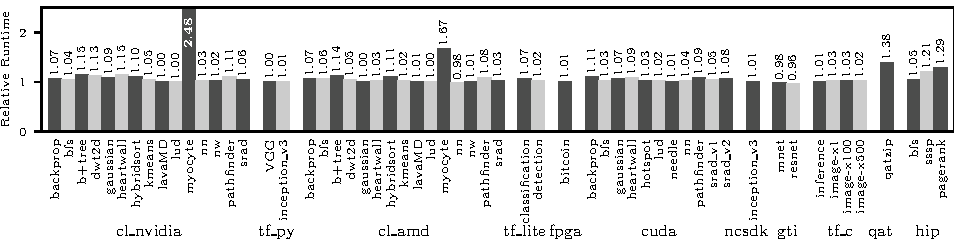
\includegraphics[width=\textwidth]{ava/data/end2end/end2end_all.pdf}
    \vspace{-1.75em}
	\caption{End-to-end execution time on virtualized APIs or accelerators normalized to native execution time. \lstinline|tf_py| is the handwritten TensorFlow Python API remoting with \AvA API-agnostic components.}
	\label{fig:end2end}
	%\vspace*{-0.75em}
\end{figure*}

\begin{figure}
	\centering
	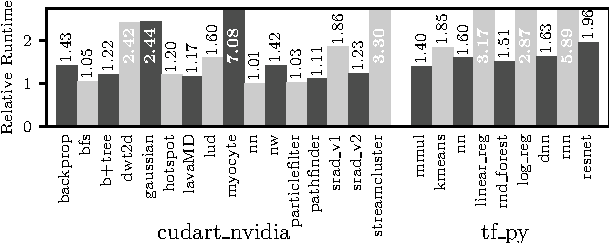
\includegraphics[width=\columnwidth]{ava/data/end2end/end2end_cudart.pdf}%
	\vspace*{-.1em}
	\caption{End-to-end execution time on virtualized CUDART and CUDA-accelerated TensorFlow APIs normalized to native execution time.}
	\label{fig:end2end_cudart}
	%\vspace*{-.6em}
\end{figure}

\begin{comment}
\amp{Move these the section that addresses them if we want to use them explicitly.}
Our evaluation focuses on:
\begin{compactitem}
\item Quantifying the development effort involved in virtualizing an accelerator API using \AvA.
\item Understanding \AvA's efficacy for different API frameworks.
\item Application performance on a \AvA-virtualized accelerator.
\item The sources of overhead in a virtual stack constructed with \AvA, and possible optimizations.
\item \AvA's ability to enforce resource policies (e.g., fair sharing).
\item The performance of \AvA's record-and-replay scheme.
\end{compactitem}
\end{comment}


\AvA was evaluated on an Intel Xeon E5-2643 CPU with 128~GiB DDR4 RAM, using
Ubuntu~18.04 LTS, and Linux 4.14 with modified KVM and vhost modules.
Guest VMs were assigned 4 virtual cores, 4~GiB memory, 30~GB disk space, and ran Ubuntu~18.04 LTS with the stock Linux 4.15 kernel.
\workers and VMs were co-located on the same server for all experiments except live migration and the FPGA benchmarks.
Experiments involving a Google Cloud TPU were carried out on a Google Compute Engine instance with 8 vCPUs (SkyLake), 10~GiB memory, and a disaggregated Cloud TPU v2-8 in the same data center.
The guest VM was located on the same instance via nested virtualization.
Experiments for the custom FPGA API were done on an AWS F1 \lstinline|f1.2xlarge| instance (with 1 Virtex UltraScale+ FPGA, 8 vCPUs, and 122 GiB memory).
For live migration, a second similar server was used as the remote machine, and the servers were directly connected by 10 Gigabit Ethernet.

\subsection{Development Effort}
\label{s:eval_effort}

%Traditional API forwarding schemes have had trouble keeping up with the rate
%of evolution of framework APIs due to the massive engineering effort needed.
%\AvA is designed to assist virtualization engineers by automatically
%generating the guestlib and \worker for each API from a specification written
%in \Lapis.

\definecolor{Gray}{gray}{0.9}
\begin{table}
	\footnotesize
    \newcolumntype{\N}{S[table-format=4.0, table-alignment = right, table-auto-round = true]}
    \newcolumntype{\n}{S[table-format=1.0, table-alignment = right, table-auto-round = true]}
    \setlength{\tabcolsep}{3pt}
	% \begin{tabular}{>{\raggedright\arraybackslash}m{7.4em}m{0.8em}\n\N\N >{\raggedright\arraybackslash}m{4.0em}>{\raggedright\arraybackslash}m{7.4em}}
	\begin{tabular}{ccccccc}
    \toprule
	API                         & Gen              & {\#}                 & {LoC}                  & {Churn}                 & Benchmark                & Hardware                                      \\
	\midrule
	\multirow{2}{*}{OpenCL~1.2} & \cross \cellcolor{Gray} & {\cellcolor{Gray}}39 & {\cellcolor{Gray}}7514 & {\cellcolor{Gray}}14318 & \multirow{2}{*}{Rodinia} & \multirow{2}{7em}{NVIDIA~GTX~1080 AMD~RX~580} \\
                                & \checkmark       & 38                   & 1060                   & 2868                    &                          &                                               \\
	CUDA 10 Driver              & \checkmark       & 16                   & 266                    & 410                     & Rodinia                  & NVIDIA~GTX~1080                               \\
	CUDA 10 Runtime             & \checkmark       & 93                   & 1358                   & 1973                    & Rodinia                  & NVIDIA~GTX~1080 								\\
	TensorFlow~1.12~C           & \checkmark       & 46                   & 501                    & 887                     & Inception                & NVIDIA~GTX~1080                               \\
	TensorFlow~1.13~Py          & \cross           & {\scriptsize n/a}    & 3245                   & 5972                    & VGG-net Inception        & Google~Cloud TPU v2-8                         \\
	TensorFlow~1.14~Py          & \checkmark       & 111                  & 1865                   & 2557                    & Neural networks          & NVIDIA~GTX~1080 								\\
	TensorFlow Lite~1.13        & \cross           & {\scriptsize n/a}    & 1295                   & 2005                    & Official examples        & Coral Edge~TPU                                \\
	NCSDK~v2                    & \checkmark       & 26                   & 479                    & 1279                    & Inception                & Movidius~NCS v1                         \\
	GTI SDK~4.4                 & \checkmark       & 38                   & 284                    & 568                     & Official examples    & Gyrfalcon 2803 Plai Plug                         \\
	Custom FPGA on AmorphOS~\cite{amorphos}     & \checkmark       & 4                    & 30                     & 40                      & BitCoin  & AWS~F1                                        \\
	QuickAssist~1.7             & \checkmark       & 19                   & 444                    & 676                     & QATzip                   & Intel~QAT 8970                      \\
	HIP                         & \checkmark       & 41                   & 624                    & 990                     & Galois~\cite{tao}        & AMD~Vega~64                                   \\
	\bottomrule
	\end{tabular}
	\caption{Development effort for forwarding different APIs, along with the benchmarks~\cite{inceptionv3,vggnet,rodinia} and hardware used to evaluate them.
      The \textbf{\#} column indicates the number of API functions supported.
      The Python APIs are forwarded dynamically, making \# inapplicable.
      \textbf{Gen} indicates whether the API forwarding was generated by \CAvA or was written by hand.
      \textbf{LoC} is the number of lines of code (including blank lines and comments) in the \CAvA specification or C/Python code.
      \textbf{Churn} is the total number of lines modified in commits.
      % Inception is Inception~v3~\cite{inceptionv3}.
      % VGG-net is from \cite{vggnet}.
      % Rodinia is from \cite{rodinia}.
    }
	\label{tab:apis-and-accelerators}
	\vspace*{-.2em}
\end{table}

\begin{comment}
\begin{table}
	\footnotesize
	\begin{tabularx}{\columnwidth}{p{8em}p{4em}P{4em}p{4em}p{4em}}
	\toprule
	API Name & \#Supported   & Generated & L.o.C. & Churn\\
	\midrule
	OpenCL~1.2               & 39    &            & 7,514 & 14,318\\
	\rowcolor{Gray}
	OpenCL~1.2               & 38    & \checkmark & 1,060 & 2,868\\
	CUDA 10.0 Driver         & 16    & \checkmark & 266   & 410\\
	\rowcolor{Gray}
	Tensorflow~1.12 (C)      & 46    & \checkmark & 501   & 887\\
	Tensorflow~1.13 (Py)     & {n/a} &            & 3,245 & 5,972\\
	\rowcolor{Gray}
	Tensorflow Lite~1.13     & {n/a} &            & 1,295 & 2,005\\
	NCSDK~v2                 & 26    & \checkmark & 479   & 1,279\\
	\rowcolor{Gray}
	Custom FPGA API          & 4     & \checkmark & 30    & 40\\
	QuickAssist~1.7          & 19    & \checkmark & 444   & 676\\
	\rowcolor{Gray}
	HIP                      & 41    & \checkmark & 624  0 & 990\\
	\bottomrule
	\end{tabularx}
	\caption{Development effort for forwarding different APIs. Number of APIs supported is not applicable to Python APIs as they are forwarded dynamically. The \textbf{Generated} column indicates whether the API forwarding was generated by \CAvA or was written by hand. \textbf{L.o.C.} is the number of lines of code in the \CAvA specification or C/Python code. \textbf{Churn} is the total number of lines modified in commits.}
	\label{tab:api-dev-effort}
\end{table}
\end{comment}


We present our experience building API remoting systems by hand and with
\CAvA as evidence of the significant reduction in developer effort
\CAvA provides.
We characterize developer effort to virtualize \numframeworks APIs and \numaccelerators devices in terms of the lines of code in the \CAvA specifications or C/Python code (\texttt{LoC} in Table~\ref{tab:apis-and-accelerators}), and the number of lines of code modified (\textbf{Churn} in Table~\ref{tab:apis-and-accelerators}) during development (counted from commits).
Building an API remoting system for OpenCL, which supports all the APIs needed to run the Rodinia~\cite{rodinia} benchmarks, by hand took more than 3 developer-months, and spanned 7,514 LoC (see row 1 of Table~\ref{tab:apis-and-accelerators}).
Supporting the same subset of OpenCL with \AvA, took a single developer a little over a week, and the resulting API specification was 1,060 LoC long.
%The reduction in both time spent and lines of code written and modified to virtualize the OpenCL API %demonstrates that \CAvA reduces the effort required to virtualize a compute accelerator API.
Even in cases where we couldn't leverage \AvA---%
TensorFlow and TensorFlow Lite Python APIs---%
leveraging \AvA's API-agnostic components enabled us to build a \hira system with reasonable effort (3,245 lines of Python code and 2 developer weeks for TensorFlow Python).

\subsection{End-to-end Performance}

% We measured the APIs and accelerators that we virtualized with \AvA using the benchmarks described in Table~\ref{tab:apis-and-accelerators}.
Figure~\ref{fig:end2end}--\ref{fig:end2end_cudart} shows the end-to-end runtime, normalized to native, for all benchmarks, accelerator and API combinations we support (see Table~\ref{tab:apis-and-accelerators}).
\AvA introduces modest overhead for most workloads.
%geometric mean overhead is 8.6\%.
Excluding \texttt{myocyte}, the Rodinia OpenCL benchmarks on NVIDIA GTX 1080
GPU slowed down by 7\% on average.
The outlier, \texttt{myocyte} has over 2$\times$ overhead because it is extremely \textbf{call-intensive}---it makes over 200,000 calls in \SI{18.5}{\second}; most others make between 30 and 3,000 calls.
For comparison, FlexDirect sees 3.3$\times$ slowdown for \texttt{myocyte};
GPUvm sees 100$\times$ or more for call-intensive workloads~\cite{yufull}.
\texttt{Myocyte} experienced lower overhead on the AMD Radeon RX
580 GPU, as the kernels executed 3$\times$ slower, allowing more of
\AvA's overheads to be amortized.
The benchmarks for CUDA runtime API and CUDA-accelerated TensorFlow are mostly call-intensive.
The geometric mean overhead is 79.6\%, 4$\times$ faster than FlexDirect.

The TensorFlow benchmarks for the handwritten Python API remoting system, and Movidius benchmarks show low overhead---%
0\% overhead on VGG-net running on TensorFlow Python (Cloud TPU), and 7\% slowdown for image classification on TensorFlow Lite (Coral Edge TPU)---%
as they are \textbf{compute-intensive}. Each offloaded kernel performs a lot of computation per byte of data transferred, with relatively few API calls.
The Gyrfalcon benchmarks enjoy a slight speedup as time spent loading and initializing the library are eliminated by using a pre-spawned \worker pool.
The QuickAssist accelerator proved challenging to virtualize, as it is a high-data-rate kernel-bypass encryption/compression accelerator.
Applications that run on this device are \textbf{data-intensive}: computation per transferred byte is very low.
We ran the Intel QATzip compression application on the Silesia corpus~\cite{silesia} using synchronous QAT APIs: while the application only experienced a 1.38$\times$ end-to-end runtime slowdown, its throughput was 2.2$\times$ lower on average.
\AvA was not able to keep up with the high throughput of the device, due to data transfer and marshalling overheads, as the time spent transferring data between the guest and the host was equivalent to compute time on the accelerator.
We are exploring zero-copy techniques to ameliorate this. We note that QAT on \AvA is fair, unlike the onboard SR-IOV support.

% QATzip with different datasets on QuickAssist API,
% for which the average end-to-end overhead is 38.8\%,
% but the throughput for data compression has 2.2$\times$ slowdown.
% \hyu{@Amogh, explain..}


% \subsubsection{Workload Characteristics}\hyu{Address when we gather up}
\label{s:micro_benchmark}

\begin{figure}
  \centering
	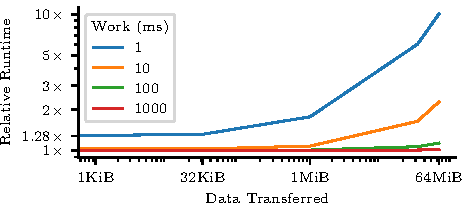
\includegraphics[width=\columnwidth]{ava/data/microbenchmark/overhead_plot.pdf}%
    \vspace*{-.5em}
	\caption{Overhead on a micro-benchmark with varying work per call and data per call. The plot is log-log and the trend is linear.
    % \aak{what is the data normalized to? How much data was computed on, i.e., does this represent call-intensive at 1KiB and data-intensive at 64MiB?}
    }
	\label{fig:microbenchmark_overhead}
	%\vspace*{-0.5em}
\end{figure}

\subsection{Micro-benchmarks}

To understand performance trade-offs for \AvA,
%suitability for compute-intensive, data-intensive, and call-intensive applications,
we ran a micro-benchmark that transferred different amounts of data per call and simulated accelerator computation for different lengths of time by spinning on the host.
Figure~\ref{fig:microbenchmark_overhead} shows compute-intensive applications (represented by the lines for 100~ms and 1,000~ms of work) suffer the lowest overhead, as data transfer is amortized by time computing on that data.
Data-intensive applications (represented by the 1~ms and 10~ms lines) experience severe slowdowns as the data transferred per call increases, such as when 64~MiB is moved for only 1~ms of compute.
Call-intensive applications transfer little data and have short kernels, so control transfer dominates execution, (e.g. 28\% overhead on 1~ms calls with no data).


\begin{comment}
\aak{commented this out cos we've expressed the same thing more compactly above.}
\paragraphbe{Compute-intensive} applications have long device computations with relatively little data transferred per call and infrequent calls.
	This kind of applications are offloading compute kernels to an accelerator with an API (e.g., OpenCL and CUDA).
    Specialized machine learning frameworks~\cite{caffe,graphcore,pytorch_use_gpu,tensorflow_use_gpu,abadi2016tensorflow,cyphers2018intel} are also compute-intensive.
    %, like Tensorflow, Caffe2, PyTorch, Poplar, Nervana, and nGraph,
	In compute-intensive APIs, the overheads of data transfer and API forwarding are amortized by the long execution time, leading to low overall overhead.\hyu{Shrink}

\paragraphbe{Data-intensive} applications have large data transfers and relatively short compute kernels,
	so the data transfer overhead cannot be amortized.
	Some OpenCL and CUDA workloads fall into this category,
	as the device compute time is much shorter than the data transfer time;
    kernel bypass APIs (e.g., Intel QAT) often fall into this category as well.
	This overhead could be reduced with zero-copy data transfer.

\paragraphbe{Call-intensive} applications have short frequent API calls.
    A common example of this is the network communication with a NIC API.
    This type of API is not suitable for API remoting, because the per call transport overhead is unacceptable.
\end{comment}

\begin{figure}[!th]
	\centering
	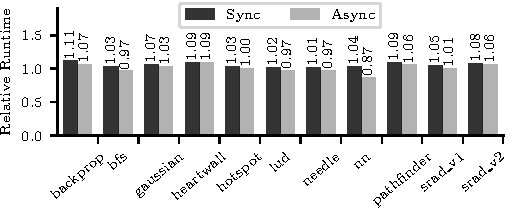
\includegraphics[width=\columnwidth]{ava/data/end2end/end2end_async.pdf}%
	\vspace*{-.5em}
	\caption{End-to-end runtime of CUDA benchmarks (relative to native) using synchronous and asynchronous specifications.}
	\label{fig:eval_async}
	\vspace*{-1em}
\end{figure}

\subsubsection{Asynchrony Optimizations}
\label{s:opt_eval}

% We measured the system using OpenCL benchmarks on NVIDIA GTX 1080 GPU with two transport channels, shared memory and VM socket, with or without asynchrony calls.
% In most cases, shared memory has obvious improvement to the performance, 20\% speedup in average,
% because VM socket with virtio-vsock device suffers from low throughput due to the limited size of receive buffers and the share of the single RX/TX virt-queue pair among all applications in the same VM.
% Benchmarks such as nw and pathfinder suffer from slowdown with shared memory,
% because they transfer small amount of data, and the cost of shared memory management cannot be counteracted by the reduction of data copies.
% \subsection{Asynchrony}
% \label{s:asynchrony}
% \AvA allows functions annotated as

% Some synchronous  may safely be executed asynchronously:
Synchronous APIs calls that have no output of any kind remain semantically correct if executed asynchronously.
For example, \lstinline|clSetKernelArg| is a synchronous OpenCL API,
but can be forwarded asynchronously to reduce the overhead of these calls. % at the cost of fidelity:
The application's execution will not be faithful to native execution, as the library would return immediately after the command is sent to the \worker.
Any resulting errors will be delivered from a later API call.
Similar techniques were applied in vCUDA (lazy RPC)~\cite{vCUDA} and rCUDA (API batching)~\cite{rCUDA}. % with the same loss of fidelity.

We annotated several synchronous APIs---\lstinline[breaklines=true,escapechar=|]@cuLaunchKer@\-\lstinline@nel@, \lstinline@cuMemcpyHtoD@, and resource free functions---as asynchronous.
% The errors in these calls may be reported in a later call,
% but successful execution produces correct results.
Figure~\ref{fig:eval_async} shows that this optimization results in a 5\% speedup on average (geometric mean) in end-to-end runtime (normalized to native) for CUDA Rodinia benchmarks.
%Several benchmarks (e.g., \textit{nn}) experience speedup because \aak{figure out why nn is so fast.} \hyu{Fix: Transfer, execution overlap; release non-blocking}.

\subsection{Scalability}
\begin{figure}
	\centering
	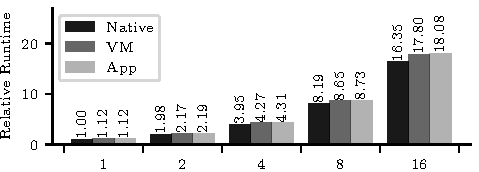
\includegraphics[width=.95\linewidth]{ava/data/scalability/scalability.pdf}%
	\vspace{-0.4em}
	\caption{Scalability of multiple VMs running a single application each, and multiple applications in a single VM,  with \AvA. Runtime is relative to running the same number of applications natively.}
	\label{fig:scalability}
	\vspace*{-.25em}
\end{figure}

% \AvA provides scalability and concurrency for simultaneous guest VMs and applications.
To evaluate scalability, we ran multiple instances of the OpenCL \texttt{gaussian} benchmark
simultaneously in a varying number of VMs with a NVIDIA GTX 1080 GPU. The \texttt{gaussian} benchmark fully saturates the GPU.
The \AvA overhead ($\sim$10\%) does not increase as the number of VMs or applications increases,
as shown by the near-perfect scaling in Figure~\ref{fig:scalability}.
The GPU kernel execution has an average 5.7\% slowdown each time the number of VMs and applications is doubled.
% , while the end-to-end performance does not change.
This slowdown is small due
better utilization of the physical device and other system resources.
%, i.e.,
% an application in one VM can utilize the GPU when other applications are not.
% \reviewer{A}{What is the intuition behind the perfect scaling?}

Accelerators without process-level protection or sharing support (e.g., Intel Movidius NCS) do not scale will with \AvA, as multiple applications attempting to use the device have to be serialized.
\AvA added modest overheads (11\%) in a case where 4 VMs were all running inception on the NCS v1. We note that \AvA still provides benefit by enabling a hypervisor to expose and share the device across guest VMs.

% \begin{comment}
\subsection{API Rate Limiting}
\label{s:eval_rate_limit}

To measure the fairness achieved by \AvA, we repeatedly executed kernels drawn from six CUDA OpenCL benchmarks in pairs simultaneously in two VMs.
 % with virtualized NVIDIA GTX 1080 GPU.
The kernels last from 1~ms to 100~ms.
Figure~\ref{fig:fairness} shows the fairness of the execution with fixed-rate polling and feedback control method in 500-ms and 1-s measurement windows.
We compute the unfairness as
$\left|t_1-t_2\right| \mathbin{/} (t_1+t_2),$
where $t_i$ is the device time used by VM$_i$ in the time window.

% With the same size of time window, it is expected to see less fairness and smaller scheduling overhead with longer kernels as the GPU kernel is non-preemptible.
For fixed-rate polling ($p=5$~ms), median unfairness in a 1~s window is 2.6\%, and scheduling overhead was 7\%.
For feedback control ($a=1$~ms and $b=1/2$),
%The initial, minimum and maximum delays are set to 5~ms, 0.5~ms and 10~ms correspondingly.
median unfairness is 2.4\% in a \SI{1}{\second} measurement window, with 15\% overhead.

\begin{figure}
	\centering
    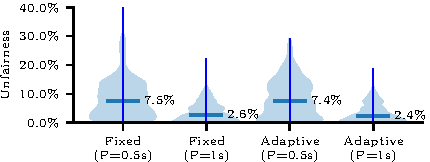
\includegraphics[width=\columnwidth]{ava/data/rate_limit/bias_plot.pdf}%
    \vspace{-.35em}
	\caption{Unfairness of the fixed and adaptive scheduling algorithms with two different measurement periods.
      The width of the shaded areas show the probability of the bias (unfairness) being a specific value in any given measurement window.
      The horizontal bar shows the median and the vertical line runs from the minimum to the maximum.}
	\label{fig:fairness}
\end{figure}


\subsection{Live Migration}

\begin{figure}
	\centering
	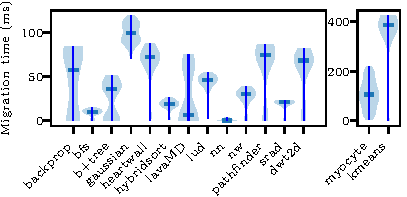
\includegraphics[width=\columnwidth]{ava/data/migration/time_plot.pdf}%
    % \vspace{-0.6em}
	% 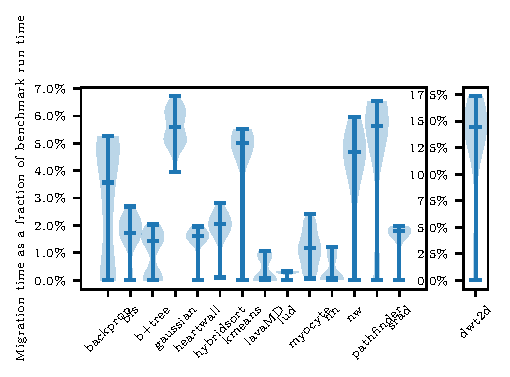
\includegraphics[width=\columnwidth]{ava/data/migration/factor_plot.pdf}
	\caption{Live migration downtime for single-threaded OpenCL benchmarks on NVIDIA GTX 1080.
      This downtime is in addition to the $\sim$\SI{75}{\milli\second} of downtime of the VM migration itself.
      Migration downtime does not include time spent waiting for executing kernels to complete (accounted as latency), as the application is still performing useful computation on the accelerator during that time.
      % The width of the shaded areas show the the probability of a migration taking that length of time.
      % The horizontal bar shows the median and the vertical line shows the range from minimum to maximum.
    }
	\label{fig:migration}
	%\vspace{-.5em}
\end{figure}

% To evaluate \AvA's
%live-migration scheme uses annotations and selective record-and-replay instead of replaying the entire application on the remote.
%To understand the efficacy of our method,
We live-migrated a VM with 4~GB memory, that was running OpenCL applications from the Rodinia benchmark suite, between two servers that were directly connected via a 10~Gib Ethernet link, both equipped with NVIDIA GTX 1080 GPUs.
Migration was triggered at random points in each benchmark, and the application could not make API calls for the duration of the migration.
Migrating the VM without \AvA or GPU usage takes \SI{19}{\second} with a \SI{75}{\milli\second} downtime on average.
% In the experiment, the migration is started at random points during the OpenCL application's lifetime,
% where the application is paused until the migration is done.
% Both servers had .

\begin{comment}
Migration was carried out in three pipelined stages:
the source \worker extracted explicit state from API objects, and then transferred recorded commands for implicit state and replacement commands for explicit state to the target \worker. The target \worker then replayed the transferred commands.
\aak{I think we don't need this here. We've already explained it in the migration section...}
\end{comment}

\begin{comment}
Migration samples for each benchmark:
backprop: 50
bfs: 50
b+tree: 50
dwt2d: 50
gaussian: 150
heartwall: 50
hybridsort: 50
kmeans: 50
lavaMD: 50
lud: 150
myocyte: 200
nn: 50
nw: 50
pathfinder: 50
srad: 50
\end{comment}

Figure~\ref{fig:migration} shows the downtime experienced by applications in the VM, not including downtime for migrating the VM itself.
200 samples were collected for \texttt{myocyte}, 150 for \texttt{gaussian} and \texttt{lud}, and 50 for all others.
% , based on the number of APIs calls made by the applications.

The dominant cost is command transfer and replay, but this cost is also affected by the size of the benchmark's state.
Figure~\ref{fig:migration} shows a bimodal distribution of downtime for most benchmarks. This is an artifact of applications allocating device memory before entering a steady execution state, and freeing it at termination.
% \amp{Don't the benchmarks also free the buffers during execution? If the buffers were ALL freed at the end I would expect a MUCH more spread out distribution.}
%\hyu{Most free buffers at the end. Gaussian and myocyte are exceptions.}
Migrations that occur before device memory allocation do not need to transfer significant state; migrations that occur after device memory allocation do.
% but migrations after buffer creation must copy all the resident buffers and their associated commands.

% Because our test servers are connected via a relatively slow TCP link, the transfer stage can be slow.
% For example, dwt2d allocates large device memory buffers, and the buffer transfer time exceeds the benchmark's length\amp{Is this still true with 10g?}.\hyu{Not true any more.}

%\aak{this paragraph is conflicting with the caption of the figure.}
%\hyu{One is downtime, one is latency.}
%\AvA needs to wait for in-flight calls to finish,
%introducing latency which can be as long as the kernel execution time in the worst case.
%The \textit{Kmeans} benchmark comprises a long-running GPU kernel, so its migration time is up to 425~ms.
%However, the pause time of the application does not include this latency, because during that time the application is still performing useful computation on the accelerator.
%For applications which must execute more than one kernel to fully utilize the device, this latency could increase the perceived downtime.

% !TeX root = proposal.tex
\section{Related Work}
\label{sec:related}

Virtualization has such a long and storied history that Attempting to capture
the entire story is an exercise in futility. The introduction~\ref{sec:intro}
captures the history of CPU virtualization in broad strokes. This section then
focuses on a major theme of the proposed dissertation:
accelerator virtualization.

Accelerating specific computation is not a new idea---support for specialized
computation is extremely commonplace in CPUs (e.g., Floating Point Units
(FPU), Vector Processing Units). These specialized compute units are
typically exposed to the programmer as extensions to the Instruction Set
Architecture (ISA). Virtualizing these specialized compute units, therefore,
is no different from virtualizing the rest of the CPU and ISA virtulaization
is well explored~\cite{cp40,vm370,popek-goldberg,bugnion-disco,
bugnion-nieh-tsafrir,bugnion-workstation}.

Processors specialized for complex computational tasks, such as graphical
rendering, largely evolved as discrete devices separate from the CPU (although
some CPUs do integrate GPUs). These devices are not typically integrated into
the CPU ISA; instead, they appear to system software as I/O devices with
memory-mapped command-queues and I/O registers. I/O virtualization is well
understood~\cite{waldspurger12cacm,paradice,Kuperman_undated-io,Sig2010-ml,
zeng2013improved,abramson2006intel}, but these techniques aren't enough to
virtualize programmable accelerators. Although programmable accelerators look
like I/O devices, they are also general computing platforms, i.e., they load
binaries, have their own memory, and are typically exposed to the application
programmer via an API.

\subsection{GPU Virtualization}

% !TeX root = proposal.tex
\def\libnomod{lib unmod\xspace}
\def\osnomod{OS unmod\xspace}
\def\sharing{sharing\xspace}
\def\isolation{isolation\xspace}
\def\scheduling{sched. policy\xspace}
\def\perf{performance\xspace}
\def\libflex{lib-compat\xspace}
\def\hwflex{hw-compat\xspace}
\def\mobility{migration\xspace}
\def\gfx{graphics\xspace}
\def\gpgpu{GPGPU\xspace}
\def\id{I/D}
\def\discrete{\emph{D}}
\def\integrated{\emph{I}}
% \def\poor{--}
% \def\good{+}
% \def\ok{+/-}
% \def\verygood{++}
% \def\verybad{-- --}
\def\poor{\textbf{poor}\xspace}
\def\good{\textbf{good}\xspace}
\def\ok{\textbf{ok}\xspace}
\def\verygood{\textbf{excellent}\xspace}
\def\verybad{\textbf{bad}\xspace}
%\def\chk{$\times$}
\def\chk{\checkmark}
\def\cross{$\times$\xspace}
\def\gr{\cellcolor[gray]{0.9}}
\def\redc{\cellcolor[gray]{0.4}}
\def\bluec{\cellcolor[gray]{0.1}}

%\newcommand{\mc}[2]{\multicolumn{#1}{c}{#2}}
\definecolor{Gray}{gray}{0.6}
\definecolor{LightCyan}{rgb}{0.88,1,1}
%\newcolumntype{a}{>{\columncolor{Gray}}c}
\def\FV{\textbf{FV}}
\def\PT{\textbf{PT}}
\def\PV{\textbf{PV}}
\def\APIR{\textbf{API-R}}
\def\unmodlib{\textbf{UL}}
\def\unmodos{\textbf{UOS}}
\def\safe{\textbf{I}}
\def\fair{\textbf{F}}
\def\mob{\textbf{M}}

\setlength{\aboverulesep}{0pt}
\setlength{\belowrulesep}{0pt}

\begin{table*}[ht!]
\vspace*{2em}
\centering
\footnotesize{
\resizebox{\textwidth}{!}{
\begin{tabular}{r|l|c|c|c|c|c|c|c|c|c|c|c|c|c|c|c|}
%\hline
\T\B {\textbf{Technique}}       &
\T\B {\textbf{System}}          &
\rot{\textbf{\libnomod}}        &
\rot{\textbf{\osnomod}}         &
\rot{\textbf{\libflex}}         &
\rot{\textbf{\hwflex}}          &
\rot{\textbf{\sharing}}         &
\rot{\textbf{\isolation}}       &
\rot{\textbf{\mobility}}        &
\rot{\textbf{\parbox{4cm}{sched. \\policy}\xspace}}      &
\rot{\textbf{\gfx}}             &
\rot{\textbf{\gpgpu}}           &
\rot{\textbf{\id}}              &
\rot{\textbf{benchmark}}        &
\rot{\textbf{slowdown}}         &
\rot{\textbf{\parbox{4cm}{native\\speedup}}}    &
\rot{\textbf{\parbox{4cm}{virtual\\speedup}}}
\\   \hline

\T\B \multirow{2}{*}{\textbf{Full-virtual}}     &
     \T\B \textbf{GPUvm~\cite{GPUvm}}           &
     \T\B \chk                                  &  % unmodified guest libraries
     \T\B                                       &  % unmodified guest OS
     \T\B \chk                                  &  % lib-compatibility
     \T\B                                       &  % hw-compatibility
     \T\B \chk                                  &  % cross-VM sharing
     \T\B \chk                                  &  % cross-VM isolation
                                                &  % VM migration
     \T\B XC, BAND                              &  % fairness
                                                &  % graphics support
     \T\B \chk                                  &  % GPGPU support
     \T\B \discrete                             &  % integrated-discrete
     \T\B Rodinia                               &  % benchmark
     \T\B 141$\times$                           &  % base slowdown
     \T\B 11.4$\times$                          &  % native speedup
     \T\B {\textcolor{red}{0.08$\times$}}          % virtualized speedup
     \\ \cline{2-17}
                                                &
     \T\B \textbf{gVirt~\cite{gVirt}}           &
     \T\B \chk                                  &  % unmodified guest libraries
     \T\B                                       &  % unmodified guest OS
     \T\B \chk                                  &  % compatibility
     \T\B                                       &  % compatibility
     \T\B \chk                                  &  % cross-VM sharing
     \T\B \chk                                  &  % cross-VM isolation
     \T\B \chk                                  &  % VM migration
     \T\B QoS                                   &  % fairness
     \T\B \chk                                  &  % graphics support
     \T\B                                       &  % GPGPU support
     \T\B \integrated                           &  % integrated-discrete
     \T\B 2D~\cite{phoronix}, 3D~\cite{cairoperf}& % benchmark
     \T\B 1.6$\times$                           &  % base slowdown
     \T\B N/A                                   &  % native speedup
     \T\B N/A                                      % virtualized speedup
     \\ \hline

\T\B \textbf{PCIe Pass-thru}                    &
     \T\B \textbf{AWS GPU~\cite{amazongpu}}     &
     \T\B \chk                                  & % unmodified guest lib
     \T\B \chk                                  & % unmodified guest OS
     \T\B \cellcolor{gray!25}                   & % compatibility
     \T\B \cellcolor{gray!25}                   & % compatibility
     \T\B \cellcolor{gray!25}                   & % sharing
     \T\B \cellcolor{gray!25}                   & % isolation
     \T\B \cellcolor{gray!25}                   & % mobility
     \T\B \cellcolor{gray!25}                   & % fairness
     \T\B \chk                                  & % graphics
     \T\B \chk                                  &  % GPGPU support
     \T\B \discrete                             &  % integrated-discrete
     \T\B Any                                   &  % benchmark
     \T\B 1$\times$                             &  % base slowdown
     \T\B \cellcolor{gray!25}                   &  % natice speedup
     \T\B \cellcolor{gray!25}                      % virtualized speedup
     \\ \hline

\T\B \multirow{4}{*}{\bf API remoting}          &
     \T\B {\bf GViM~\cite{gupta2009gvim}}       &
     \T\B                                       &  % unmodified guest libraries
     \T\B                                       &  % unmodified guest OS
     \T\B                                       &  % lib-compatibility
     \T\B \chk                                  &  % hw-compatibility
     \T\B \chk                                  &  % cross-VM sharing
     \T\B \chk                                  &  % cross-VM isolation
                                                &  % VM migration
     \T\B RR, XC                                &  % fairness
                                                &  % graphics support
     \T\B \chk                                  &  % GPGPU support
     \T\B \discrete                             &  % integrated-discrete
     \T\B CUDA 1.1 SDK                          &  % benchmark
     \T\B 1.16$\times$                          &  % base slowdown
     \T\B 22$\times$                            &  % native speedup
     \T\B {\textcolor{blue}{19$\times$}}           % virtualized speedup
     \\ \cline{2-17}


                                                &
     \T\B {\bf gVirtuS~\cite{gVirtuS}}          &
     \T\B                                       &  % unmodified guest libraries
     \T\B                                       &  % unmodified guest OS
     \T\B                                       &  % lib-compatibility
     \T\B \chk                                  &  % hw-compatibility
     \T\B \chk                                  &  % cross-VM sharing
     \T\B \chk                                  &  % cross-VM isolation
                                                &  % VM migration
     \T\B RR                                    &  % fairness
                                                &  % graphics support
     \T\B \chk                                  &  % GPGPU support
     \T\B \discrete                             &  % integrated-discrete
     \T\B CUDA 2.3 MM                           &  % benchmark
     \T\B 3.1$\times$                           &  % base slowdown
     \T\B 11.1$\times$                          &  % native speedup
%     \T\B 3.6$\times$                              % virtualized speedup
     \T\B {\textcolor{blue}{3.6$\times$}}          % virtualized speedup
     \\ \cline{2-17}

                                                &
     \T\B \T\B {\bf vCUDA~\cite{shi2012vcuda}}         &
     \T\B                                       &  % unmodified guest libraries
     \T\B \chk                                  &  % unmodified guest OS
     \T\B                                       &  % lib-compatibility
     \T\B \chk                                  &  % hw-compatibility
     \T\B                                       &  % cross-VM sharing
     \T\B                                       &  % cross-VM isolation
     \T\B \chk                                  &  % VM migration
     \T\B HW                                    &  % fairness
                                                &  % graphics support
     \T\B \chk                                  &  % GPGPU support
     \T\B \discrete                             &  % integrated-discrete
     \T\B CUDA 4.0 SDK                          &  % benchmark
     \T\B 1.91$\times$                          &  % base slowdown
     \T\B 6$\times$                            &  % native speedup
     \T\B {\textcolor{blue}{3.1$\times$}}          % virtualized speedup
     \\ \cline{2-17}

                                                &
     \T\B {\bf vmCUDA~\cite{vmCUDA}}            &
     \T\B                                       &  % unmodified guest libraries
     \T\B \chk                                  &  % unmodified guest OS
     \T\B                                       &  % lib-compatibility
     \T\B \chk                                  &  % hw-compatibility
     \T\B \chk                                  &  % cross-VM sharing
     \T\B                                       &  % cross-VM isolation
     \T\B                                       &  % VM migration
     \T\B HW                                    &  % fairness
                                                &  % graphics support
     \T\B \chk                                  &  % GPGPU support
     \T\B \discrete                             &  % integrated-discrete
     \T\B CUDA 5.0 SDK                          &  % benchmark
     \T\B 1.04$\times$                          &  % base slowdown
     \T\B 33$\times$                            &  % native speedup
     \T\B {\textcolor{blue}{31.7$\times$}}         % virtualized speedup
     \\ \hline


\T\B \multirow{4}{*}{\bf \shortstack[r]{Distributed\\API remoting}}  &
    \T\B {\bf rCUDA~\cite{rCUDA, rCUDAnew}}     &
     \T\B                                       &  % unmodified guest libraries
     \T\B \chk                                  &  % unmodified guest OS
     \T\B                                       &  % lib-compatibility
     \T\B \chk                                  &  % hw-compatibility
     \T\B \chk                                  &  % cross-VM sharing
     \T\B \chk                                  &  % cross-VM isolation
     \T\B                                       &  % VM migration
     \T\B RR                                    &  % fairness
                                                &  % graphics support
     \T\B \chk                                  &  % GPGPU support
     \T\B \discrete                             &  % integrated-discrete
     \T\B CUDA 3.1 SDK                          &  % benchmark
     \T\B 1.83$\times$                          &  % base slowdown
     \T\B 49.8$\times$                          &  % native speedup
     \T\B {\textcolor{blue}{27.2$\times$}}         % virtualized speedup
     \\ \cmidrule{2-17}

                                                &
    \T\B {\bf GridCuda~\cite{GridCuda}}         &
     \T\B                                       &  % unmodified guest libraries
     \T\B \chk                                  &  % unmodified guest OS
     \T\B                                       &  % lib-compatibility
     \T\B \chk                                  &  % hw-compatibility
     \T\B \chk                                  &  % cross-VM sharing
     \T\B \chk                                  &  % cross-VM isolation
     \T\B                                       &  % VM migration
     \T\B FIFO                                  &  % fairness
                                                &  % graphics support
     \T\B \chk                                  &  % GPGPU support
     \T\B \discrete                             &  % integrated-discrete
     \T\B CUDA MM, SOR                          &  % benchmark
     \T\B 1.23$\times$                          &  % base slowdown
     \T\B \cellcolor{gray!10}                   &  % native speedup
     \T\B \cellcolor{gray!10}                      % virtualized speedup
     \\ \cmidrule{2-17}

                                                &
    \T\B {\bf SnuCL~\cite{kim2012snucl}}        &
     \T\B                                       &  % unmodified guest libraries
     \T\B \chk                                  &  % unmodified guest OS
     \T\B                                       &  % compatibility
     \T\B                                       &  % compatibility
     \T\B \chk                                  &  % cross-VM sharing
     \T\B \chk                                  &  % cross-VM isolation
     \T\B                                       &  % VM migration
     \T\B \cellcolor{gray!25}                   &  % fairness
                                                &  % graphics support
     \T\B \chk                                  &  % GPGPU support
     \T\B \discrete                             &  % integrated-discrete
     \T\B SNU NPB~\cite{seo2011performance}     &  % benchmark
     \T\B \cellcolor{gray!25}                   &  % base slowdown
     \T\B \cellcolor{gray!10}                   &  % native speedup
     \T\B \cellcolor{gray!25}                      % virtualized speedup
     \\ \cmidrule{2-17}

                                                &
    \T\B {\bf VCL~\cite{VCL}}                   &
     \T\B                                       &  % unmodified guest libraries
     \T\B \chk                                  &  % unmodified guest OS
     \T\B                                       &  % lib-compatibility
     \T\B \chk                                  &  % hw-compatibility
     \T\B \chk                                  &  % cross-VM sharing
     \T\B \chk                                  &  % cross-VM isolation
     \T\B                                       &  % VM migration
     \T\B \cellcolor{gray!25}                   &  % fairness
                                                &  % graphics support
     \T\B \chk                                  &  % GPGPU support
     \T\B \discrete                             &  % integrated-discrete
     \T\B Stencil2D~\cite{danalis2010scalable}  &  % benchmark
     \T\B \cellcolor{gray!25}                   &  % base slowdown
     \T\B \cellcolor{gray!10}                   &  % native speedup
     \T\B \cellcolor{gray!25}                      % virtualized speedup
%     \T\B {\textcolor{blue}{3.4$\times$}}          % virtualized speedup
     \\ \hline

\T\B \multirow{7}{*}{\textbf{Para-virtual}} &
     \T\B \textbf{GPUvm~\cite{GPUvm}}           &
     \T\B                                       &  % unmodified guest libraries
     \T\B                                       &  % unmodified guest OS
     \T\B                                       &  % compatibility
     \T\B                                       &  % compatibility
     \T\B \chk                                  &  % cross-VM sharing
     \T\B \chk                                  &  % cross-VM isolation
                                                &  % VM migration
     \T\B XC, BAND                              &  % fairness
                                                &  % graphics support
     \T\B \chk                                  &  % GPGPU support
     \T\B \discrete                             &  % integrated-discrete
     \T\B Rodinia                               &  % benchmark
     \T\B 5.9$\times$                           &  % base slowdown
     \T\B 11.4$\times$                          &  % native speedup
     \T\B {\textcolor{blue}{1.9$\times$}}          % virtualized speedup
     \\ \cmidrule{2-17}

                                               &
    \T\B {\bf HSA-KVM~\cite{kaveri16vee}}      &
    \T\B \chk                                  &  % unmodified guest libraries
    \T\B                                       &  % unmodified guest OS
    \T\B                                       &  % compatibility
    \T\B                                       &  % compatibility
    \T\B \chk                                  &  % cross-VM sharing
    \T\B \chk                                  &  % cross-VM isolation
                                               &  % VM migration
    \T\B HW                                    &  % fairness
    &  % graphics support
    \T\B \chk                                  &  % GPGPU support
    \T\B \integrated                           &  % integrated-discrete
    \T\B AMD OCL SDK                           &  % benchmark
    \T\B 1.1$\times$                           &  % base slowdown
    \T\B \cellcolor{gray!10}                   &  % native speedup
    \T\B \cellcolor{gray!10}                      % virtualized speedup
    \\ \cline{2-17}
                                                &
     \T\B {\bf LoGV~\cite{logv}}                &
     \T\B \chk                                  &  % unmodified guest libraries
     \T\B                                       &  % unmodified guest OS
     \T\B \chk                                  &  % compatibility
     \T\B                                       &  % compatibility
     \T\B \chk                                  &  % cross-VM sharing
     \T\B \chk                                  &  % cross-VM isolation
     \T\B \chk                                  &  % VM migration
     \T\B RR                                    &  % fairness
     \T\B                                       &  % graphics support
     \T\B \chk                                  &  % GPGPU support
     \T\B \discrete                             &  % integrated-discrete
     \T\B Rodinia                               &  % benchmark
     \T\B 1.01$\times$                          &  % base slowdown
     \T\B 11.4$\times$                          &  % native speedup
     \T\B {\textcolor{blue}{11.3$\times$}}         % virtualized speedup
     \\ \cmidrule{2-17}

                                                &
     \T\B \textbf{SVGA2~\cite{dowty2009gpu}} &
     \T\B \chk                                  &  % unmodified guest libraries
     \T\B                                       &  % unmodified guest OS
     \T\B                                       &  % compatibility
     \T\B                                       &  % compatibility
     \T\B \chk                                  &  % cross-VM sharing
     \T\B \chk                                  &  % cross-VM isolation
     \T\B \chk                                  &  % VM migration
     \T\B \cellcolor{gray!25}                   &  % fairness
     \T\B \chk                                  &  % graphics support
                                                &  % GPGPU support
     \T\B \discrete                             &  % integrated-discrete
     \T\B 2D, gaming                            &  % benchmark
     \T\B 3.9$\times$                           &  % base slowdown
     \T\B \cellcolor{gray!25}                   &  % native speedup
     \T\B \cellcolor{gray!25}                      % virtualized speedup
     \\ \cmidrule{2-17}

                                                &
     \T\B \textbf{Paradice~\cite{paradice}}     &
     \T\B \chk                                  &  % unmodified guest libraries
     \T\B                                       &  % unmodified guest OS
     \T\B \chk                                  &  % compatibility
     \T\B                                       &  % compatibility
     \T\B \chk                                  &  % cross-VM sharing
     \T\B \chk                                  &  % cross-VM isolation
                                                &  % VM migration
     \T\B HW, QoS                               &  % fairness
     \T\B \chk                                  &  % graphics support
     \T\B \chk                                  &  % GPGPU support
     \T\B \discrete                             &  % integrated-discrete
     \T\B OpenGL, OpenCL                        &  % benchmark
     \T\B 1.1$\times$                           &  % base slowdown
     \T\B \cellcolor{gray!10}                   &  % native speedup
     \T\B \cellcolor{gray!10}                      % virtualized speedup
     \\ \cmidrule{2-17}

                                                &
     \T\B \textbf{VGVM~\cite{vasila-gvm16}}     &
     \T\B                                       &  % unmodified guest libraries
     \T\B                                       &  % unmodified guest OS
     \T\B                                       &  % compatibility
     \T\B \chk                                  &  % compatibility
     \T\B \chk                                  &  % cross-VM sharing
     \T\B \chk                                  &  % cross-VM isolation
                                                &  % VM migration
     \T\B HW                                    &  % fairness
                                                &  % graphics support
     \T\B \chk                                  &  % GPGPU support
     \T\B \discrete                             &  % integrated-discrete
     \T\B CUDA 5.0 SDK                          &  % benchmark
     \T\B 1.02$\times$                          &  % base slowdown
     \T\B 33$\times$                            &  % native speedup
     \T\B {\textcolor{blue}{32.3$\times$}}         % virtualized speedup
     \\ \hline

\end{tabular}
}
}
\caption{Existing GPU virtualization proposals, grouped by approach. Previously published in the Trillium paper~\cite{trillium}.}
\label{tab:virt-comp-proposal}
% \vspace*{-6pt}
\end{table*}

GPU virtualization has received a lot of attention since the late 2000s. This
section presents an overview of all prior work.
Table~\ref{tab:virt-comp} presents a comprehensive overview of prior
accelerator virtualization techniques in terms of traditional virtualization
properties. The \textbf{\libnomod} and \textbf{\osnomod}
columns indicate ability to support unmodified guest libraries and OS/driver.
The \textbf{\libflex} and \textbf{\hwflex} indicate the ability
(compatibility) to support a GPU device abstraction that is independent of
\textit{framework} or \textit{hardware} actually present on the host.
\textbf{\sharing}, \textbf{\isolation}
and \textbf{\scheduling} indicate cross-domain sharing, isolation and
some attempt to support fairness or performance isolation
(policies such as RR Round-Robin, XC XenoCredit, HW hardware-managed, etc.).
The \textbf{\mobility} shows support for VM migration.
\textbf{I/D} indicates it supports either integrated or discrete GPU. The
table also includes performance entries for each system including the
geometric-mean slowdown (execution time relative to native execution) across
all reported benchmarks. We additionally include the benchmarks used, and
where possible, a report (or estimate) of the geometric-mean speedup one
should \emph{expect} for using GPUs over CPUs using hardware similar to that
used in this paper. The final column is the expected geometric-mean speedup
for the given benchmarks running in the virtual GPGPU system over running on
native CPUs. Values in this column were computed by dividing the expected
speedup from using a GPU by the slowdown introduced by virtualization.
Entries where overheads eclipse GPU-based performance gains are marked in
\textcolor{red}{red}. Performance profitable entries are
\textcolor{blue}{blue}. \textcolor{darkgray}{Greyed out cells} indicate the
metric is meaningless for that design. \textcolor{gray}{Light grey cells}
indicate that the data was not available.


{\noindent \bf \large Full Virtualization}

\paragraphbe{GPUvm}~\cite{suzuki2014gpuvm} virtualizes CUDA on Kepler and
Fermi (NVIDIA) GPUs for Xen. GPUvm presents a GPU device model to each VM.
Attempts to access the GPU from all VMs are routed through a GPU Aggregator.
The aggregator maintains shadow page tables, shadow channels, implements a
``fair share scheduler'', and modifies requests to enforce isolation. GPUvm
interposes on communication between guest device driver and the GPU device
model, by trapping and forwarding MMIO writes. The authors also explore a
number of optimizations: lazy shadowing, bar remap, para-virtualization, and
multi-call batching. Despite these optimizations, GPUvm remains non-viable due to its high overhead---the most optimal configuration of GPUvm induces a 6~$\times$ slowdown on average.

\paragraphbe{gVirt}~\cite{tian2014full} is a \emph{graphics}-only
virtualization technique for Intel GPUs. The GPU is multiplexed among multiple
VMs via pass-through for access to performance critical resources (command
buffer and frame buffer), and trap-emulate for resources generally accessed
off the critical path (PTEs, I/O Registers). Initialization and power
management are done by the native driver in DOM0. Memory is multiplexed with a
combination of partitioning and `` ballooning''. gVirtus is geared toward
graphics and can't be easily extened to support GPGPU computing.

{\noindent \bf \large API Remoting}

\paragraphbe{GViM}~\cite{gupta2009gvim} supports a straightforward
split-driver API remoting approach to virtualization of CUDA in Xen.
CUDA API calls made by applications in the Guest VM are interposed through a
front-end driver (using Xen event channels) and forwarded to a back-end driver
in DOM0, which exercises the CUDA driver and runtime. While GViM's
split-driver design is very similar to AvA's HIRA, AvA presents an
accelerator-agnostic framework that can be used to implement
hypervisor-mediated API-remoting for arbitrary devices, can enforce flexible
policies via callbacks and tackles the compatibility issues inherent in
API-remoting.

\paragraphbe{vCUDA}~\cite{vCUDA} is another CUDA API-remoting system.
CUDA API calls are redirected through an interposer library (``vCUDA'') to a
stub in the host OS, which interacts with the device using pass through. RPC
turns out to be the primary performance term. The authors explores RPC
batching as an optimization. The system has no support for interposition.

\paragraphbe{vmCUDA}~\cite{vmCUDA} observes that while pass-through is
performant, it precludes sharing, and VM migration.
vmCUDA employs a split-driver model with a front-end driver in the guest that
provides an interposition point, and a back-end driver in the control domain
which interacts with the CUDA runtime and driver. CUDA applications in the
guest are linked against an interposer library which forward calls and data to
the appliance VM. As with vCUDA, the system guarantees no isolation among VMs.

\paragraphbe{gVirtuS}~\cite{gVirtuS} is an API remoting framework that claims
to provide transparent support for CUDA, OpenCL, and OpenGL on Xen, KVM, and
VMware ESXi, using a split-driver design to provide a formal abstraction layer
for GPUs that is independent of VMM.

\paragraphbe{rCUDA}~\cite{rCUDA, rCUDAnew},
\textbf{\textit{GridCuda}}~\cite{GridCuda},
\textbf{\textit{SnuCL}}~\cite{kim2012snucl} and
\textbf{\textit{VCL}}~\cite{VCL} are all user-mode middle-ware systems for
multiplexing GPUs and CUDA/OpenCL across a cluster. A client library
encapsulates access to a (potentially) remote GPU. While the basic design is
isomorphic to the API remoting design, virtual machines need not be present.

{\noindent \bf \large Para-virtualization}

\paragraphbe{LoGV}~\cite{logv} describes an approach to GPGPU virtualization
that uses GPU protection hardware in the hypervisor to enforce cross-VM
isolation. This strategy has two important consequences. First, cross-VM
isolation is easy to enforce, and the overheads of virtualization induced by
the hypervisor component is minimal. Second, guests are left with no hardware
mechanism to enforce cross-process isolation, which pushes the responsibility
on the guest driver, which may be forced to use high overhead techniques to
provide such guarantees. We classify LoGV as a para-virtualization technique
because it ultimately forces change on the guest OS in the form of changes to
support process isolation. The virtualization overheads reported in the paper
are exceptionally rosy (indeed, the virtualized solution is faster than native
in 3 of 4 reported benchmarks). However, the evaluation prototype makes no
effort to enforce isolation in guests, which ultimately hides a significant
cost and makes the reported numbers meaningless.

\paragraphbe{HSA-KVM}~\cite{kaveri16vee} is a para-virtual system for
Heterogeneous System Architecture (HSA) compliant systems. HSA has the CPU and
GPU integrated into the same physical address space. The GPU exposes multiple
Architected Queues (Command Queues) that can be allocated to different guests.
HSA-KVM comes closest to the flexibility, compatibility and performance of CPU
virtualization. However, the design espoused requires high levels of
co-operation from the accelerator hardware, and as alluded earlier, this level
of hardware support is still missing in most accelerators.

\paragraphbe{SVGA2}~\cite{dowty2009gpu} is VMware's \emph{graphics-only} GPU
virtualization scheme. SVGA2 employs a para-virtual split-driver design with a
custom GPU ISA for shader programs (TGSI). SVGA2 supports multiple front-end
libraries (OpenGL, DirectX, etc.) via a common driver that is shipped with
most mainstream operating systems. SVGA2 uses DirectX as an internal transport
mechanism, effectively realizing API-remoting through the split-driver design.
Trillium attempts to extend the SVGA2 model to GPGPU computing. We find that
the SVGA2 model is a poor fit for general purpose accelerators due to
drastically different constraints. As an example, consider performance. SVGA2
has a much lower target to hit: frames per second (fps), while GPGPU
virtualization must preserve the raw speedup over computing with a CPU.
This makes the multiple translations needed to implement the many-to-many
multiplexing viable for graphics rendering but not for general purpose
computation.

\subsection{Language-level Virtualization}
\textbf{\textit{Dandelion}}~\cite{dandelion} abstracts accelerators at the
language runtime by compiling sequential .Net code to the accelerator
(GPU or FPGA). vTask draws inspiration from the buffer management in Dandelion
and PTask~\cite{rossbach2011ptask}, the underlying accelerator abstraction
layer.
\textbf{\textit{HPVM}}~\cite{HPVM} explores the design of a virtual ISA
(vISA) for abstracting heterogeneous compute devices. The HPVM vISA serves as
a portable compilation target for managed language run-times built on top of
the LLVM compiler infrastructure. HPVM can serve as a replacement for LLVM in
Trillium. HPVM, however, doesn't absolve the language run-time implementation
from interacting with the accelerator silo. \textbf{\textit{TornadoVM}} is an
example of such a managed language runtime implementation (Graal VM).
% !TeX root = dissertation.tex
\chapter{Conclusion}
\label{chptr:conclusion}
\input{sections/acks}
% \ifthenelse{\boolean{publicversion}}{}{
   % % !TeX root = ../dissertation.tex
\section{Playground}
\label{sec_playground}

\subsection{Performance comparisons}

\paragraph{Metrics} Init, HtoD (MemAlloc+HtoD), Kernel, DtoH, Close. We
combine MemAlloc and HtoD time because some benchmarks use asynchronous
copy.

\paragraph{OpenCL vs CUDA} We implemented the same algorithms using
OpenCL and CUDA APIs, and compared their performance. Our experiments
show that OpenCL and CUDA runtime have similar kernel execution and
memory copy time, but OpenCL needs longer initialization time mainly for
kernel JIT compilation. Gdev has internal kernel scheduling and leads to
20x slow down.

\begin{verbatim}
gaussian 1024

gdev
Init: 25.707001
MemAlloc: 0.120000
HtoD: 9.001000
Exec: 8300.752930
DtoH: 12.928000
Close: 2.024000
Total: 8350.535156

ocl
Init: 483.151001
MemAlloc: 0.012000
HtoD: 1.602272
Exec: 421.954773
DtoH: 1.446976
Close: 0.257000
Total: 1008.859985

cuda
Exec: 425.878
Total: 517.747
\end{verbatim}

\paragraph{Full virtualization} Report relative runtime compared with
native. At least we have GPUvm running CUDA benchmarks, and we can use
the relative time to represent the overhead of full virtualization. The
data are put in \texttt{gpuvm\_cuda\_small.txt} and
\texttt{gpuvm\_cuda\_native\_small.txt}.

\paragraph{Native performance} Run OpenCL benmarks on native GPU (Quadro
6000 and Pascal 6000) as well as Intel CPU.

% }

\label{last_page}
\clearpage

%
% The next two lines define the bibliography style to be used, and the bibliography file.
\input{confnames}
\interlinepenalty=10000
\bibliographystyle{ACM-Reference-Format}
\bibliography{bib/extracted}{}
% \bibliography{bib/bibliography,bib/vgpu}{}

%\beginchanged
\newpage
\appendix
\input{artifact_eval_appendix}
%% -*- fill-column: 85; -*-
%!TEX root = ../dissertation.tex

\section{\CAvA Generated Code}
\label{app:cuMemcpyHtoD-code}

This appendix shows the generated code for the CUDA driver API function \lstinline|cuMemcpyHtoD|.
The specification used is:

\begin{lstlisting}[language=C,columns=flexible]
#include <cuda.h>
ava_type(CUdeviceptr) { ava_handle; }
CUresult CUDAAPI
cuMemcpyHtoD(CUdeviceptr dst,
             const void *src,
             size_t size) {
  ava_argument(src) {
    ava_in; ava_buffer(size);
    ava_lifetime_call; } }
\end{lstlisting}

An added \lstinline|_v2| appears throughout the generated code because the CUDA header defines \lstinline|cuMemcpyHtoD| to \lstinline|cuMemcpyHtoD_v2| as a form of symbol versioning.

\amp{I don't expect we will actually want to include this appendix in the paper, but I thought I would add it to the working draft so we can see it and extract things from it. As such I have made no attempt to format it well.}


\subsection{Structures}

The types used to transmit calls.


\begin{lstlisting}[language=C,columns=flexible]
struct cu_cu_memcpy_hto_d_v2_call {
    struct command_base base;
    intptr_t __call_id;
    CUdeviceptr dst;
    size_t size;
    void *src;
};
struct cu_cu_memcpy_hto_d_v2_ret {
    struct command_base base;
    intptr_t __call_id;
    CUresult ret;
};
struct cu_cu_memcpy_hto_d_v2_call_record {
    CUdeviceptr dst;
    size_t size;
    void *src;
    CUresult ret;
    char __handler_deallocate;
    volatile char __call_complete;
};
\end{lstlisting}

\subsection{The Application-side Stub Function}

The call stub in the application:

\begin{lstlisting}[language=C,columns=flexible]
EXPORTED CUresult
cuMemcpyHtoD(CUdeviceptr dst, const void *src, size_t size)
{
    const int ava_is_in = 1,
        ava_is_out = 0;
    intptr_t __call_id = ava_get_call_id(&__ava_endpoint);
    GPtrArray *__ava_alloc_list_cuMemcpyHtoD_v2 =
        g_ptr_array_new_full(0, (GDestroyNotify) ava_buffer_with_deallocator_free);
    size_t __total_buffer_size = 0;
    {
        /* Size: const void * src */
        if ((src) != (NULL) && (size) > (0)) {
            __total_buffer_size += command_channel_buffer_size(__chan, ((size_t)(size)) * sizeof(const void));
        }
    }
    struct cu_cu_memcpy_hto_d_v2_call *__cmd =
        (struct cu_cu_memcpy_hto_d_v2_call *)command_channel_new_command(__chan,
        sizeof(struct cu_cu_memcpy_hto_d_v2_call), __total_buffer_size);
    __cmd->base.api_id = CU_API;
    __cmd->base.command_id = CALL_CU_CU_MEMCPY_HTO_D_V2;
    __cmd->base.thread_id = shadow_thread_id(nw_shadow_thread_pool);
    __cmd->__call_id = __call_id;
    /* Input: CUdeviceptr dst */
    __cmd->dst = dst;
    /* Input: const void * src */
    if ((src) != (NULL) && (size) > (0)) {
        __cmd->src =
            (void *)command_channel_attach_buffer(__chan, (struct command_base *)__cmd, src,
            ((size_t)(size)) * sizeof(const void));
    } else {
        __cmd->src = NULL;
    }
    /* Input: size_t size */
    __cmd->size = size;
    struct cu_cu_memcpy_hto_d_v2_call_record *__call_record =
        (struct cu_cu_memcpy_hto_d_v2_call_record *)calloc(1, sizeof(struct cu_cu_memcpy_hto_d_v2_call_record));
    __call_record->dst = dst;
    __call_record->size = size;
    __call_record->src = src;
    __call_record->__call_complete = 0;
    __call_record->__handler_deallocate = 0;
    ava_add_call(&__ava_endpoint, __call_id, __call_record);
    command_channel_send_command(__chan, (struct command_base *)__cmd);
    g_ptr_array_unref(__ava_alloc_list_cuMemcpyHtoD_v2);        /* Deallocate all memory in the alloc list */
    shadow_thread_handle_command_until(nw_shadow_thread_pool, __call_record->__call_complete);
    CUresult ret;
    ret = __call_record->ret;
    free(__call_record);
    return ret;
}
\end{lstlisting}

\subsection{\Worker-side Call Handler}
The \worker handler for calls sent by the stub.
The wrapper function \lstinline|__wrapper_cuMemcpyHtoD_v2| is used to guarantee a separate scope for some of the generated code and allow \lstinline|return| to behave as expected.

\begin{lstlisting}[language=C,columns=flexible]
static CUresult
__wrapper_cuMemcpyHtoD_v2(CUdeviceptr dst, size_t size, const void *src) {
    CUresult ret;
    ret = cuMemcpyHtoD_v2(dst, src, size);
    return ret;
}

void
__handle_command_cu(struct command_channel *__chan, struct nw_handle_pool *handle_pool,
    struct command_channel *__log, const struct command_base *__cmd)
{
    int ava_is_in,
     ava_is_out;
    switch (__cmd->command_id) {
    case CALL_CU_CU_MEMCPY_HTO_D_V2:{
        ava_is_in = 1;
        ava_is_out = 0;
        GPtrArray *__ava_alloc_list_cuMemcpyHtoD_v2 =
            g_ptr_array_new_full(0, (GDestroyNotify) ava_buffer_with_deallocator_free);
        struct cu_cu_memcpy_hto_d_v2_call *__call = (struct cu_cu_memcpy_hto_d_v2_call *)__cmd;
        assert(__call->base.api_id == CU_API);
        assert(__call->base.command_size == sizeof(struct cu_cu_memcpy_hto_d_v2_call)
            &&
            "Command size does not match ID. (Can be caused by incorrectly computed buffer sizes, expecially using `strlen(s)` instead of `strlen(s)+1`)");
        /* Unpack and translate arguments */
        /* Input: CUdeviceptr dst */
        CUdeviceptr dst;
        dst = (CUdeviceptr) __call->dst;
        dst = (CUdeviceptr) nw_handle_pool_deref(handle_pool, (void *)__call->dst);
        /* Input: size_t size */
        size_t size;
        size = (size_t)__call->size;
        size = __call->size;
        /* Input: const void * src */
        void *src;
        src =
            ((__call->src) != (NULL)) ? ((const void *)command_channel_get_buffer(__chan, __cmd,
                __call->src)) : ((const void *)__call->src);
        if ((__call->src) != (NULL)) {
            void *__src_src_0;
            __src_src_0 = src;
            size_t __buffer_size;
            __buffer_size = ((size_t)(size));
            src = (const void *)command_channel_get_buffer(__chan, __cmd, __call->src);
         if ((src) != (__src_src_0)) {
                memcpy(src, __src_src_0, __buffer_size * sizeof(const void));
            }
        } else {
            src =
                ((__call->src) != (NULL)) ? ((const void *)command_channel_get_buffer(__chan, __cmd,
                    __call->src)) : ((const void *)__call->src);
        }
        /* Perform Call */
        CUresult ret;
        ret = __wrapper_cuMemcpyHtoD_v2(dst, size, src);
        ava_is_in = 0;
        ava_is_out = 1;
        size_t __total_buffer_size = 0;
        struct cu_cu_memcpy_hto_d_v2_ret *__ret =
            (struct cu_cu_memcpy_hto_d_v2_ret *)command_channel_new_command(__chan,
            sizeof(struct cu_cu_memcpy_hto_d_v2_ret), __total_buffer_size);
        __ret->base.api_id = CU_API;
        __ret->base.command_id = RET_CU_CU_MEMCPY_HTO_D_V2;
        __ret->base.thread_id = __call->base.thread_id;
        __ret->__call_id = __call->__call_id;
        /* Output: CUresult ret */
        __ret->ret = ret;
        /* Send reply message */
        command_channel_send_command(__chan, (struct command_base *)__ret);
        g_ptr_array_unref(__ava_alloc_list_cuMemcpyHtoD_v2);    /* Deallocate all memory in the alloc list */
        break;
    }
    default:
        abort_with_reason("Received unsupported command");
    }                                            // switch
}
\end{lstlisting}

\subsection{The Application-side Reply Handler}

The handler for replies from the \worker to the application:

\begin{lstlisting}[language=C,columns=flexible]
void
__handle_command_cu(struct command_channel *__chan, struct nw_handle_pool *handle_pool,
    struct command_channel *__log, const struct command_base *__cmd)
{
    int ava_is_in,
     ava_is_out;
    switch (__cmd->command_id) {
    case RET_CU_CU_MEMCPY_HTO_D_V2:{
        ava_is_in = 0;
        ava_is_out = 1;
        struct cu_cu_memcpy_hto_d_v2_ret *__ret = (struct cu_cu_memcpy_hto_d_v2_ret *)__cmd;
        assert(__ret->base.api_id == CU_API);
        assert(__ret->base.command_size == sizeof(struct cu_cu_memcpy_hto_d_v2_ret)
            &&
            "Command size does not match ID. (Can be caused by incorrectly computed buffer sizes, especially using `strlen(s)` instead of `strlen(s)+1`)");
        struct cu_cu_memcpy_hto_d_v2_call_record *__local =
            (struct cu_cu_memcpy_hto_d_v2_call_record *)ava_remove_call(&__ava_endpoint, __ret->__call_id);
        CUdeviceptr dst;
        dst = __local->dst;
        size_t size;
        size = __local->size;
        void *src;
        src = __local->src;
        CUresult ret;
        ret = (CUresult) __ret->ret;
        /* Output: CUresult ret */
        __local->ret = __ret->ret;
        __local->__call_complete = 1;
        if (__local->__handler_deallocate) {
            free(__local);
        }
        break;
    }

    default:
        abort_with_reason("Received unsupported command");
    } // switch
}
\end{lstlisting}

\end{document}
